\documentclass[a0]{sciposter}
\usepackage{lipsum}
\usepackage{epsfig}
\usepackage{mhchem}
\usepackage{amsmath}
\usepackage{amssymb}
\usepackage{multicol}
\usepackage{graphicx,url}
\usepackage[spanish]{babel}   
\usepackage[utf8]{inputenc}
%\usepackage{fancybullets}
\usepackage[backend=bibtex, style=chem-acs, natbib=true]{biblatex} 

\addbibresource{../Tesis/bibliography.bib} % The filename of the bibliography
\AtBeginBibliography{\footnotesize}

\newcommand{\groupname}{\textbf{Termodinámica de Soluciones}}
\newcommand{\grad}{$^\circ$C}
\newcommand{\figwidth}{0.7\linewidth}

\title{Puesta en marcha y calibración de un	calorímetro\\ 2277 de ThermoMetric}
%Título do projeto

\author{Juan \textsc{Barbosa}\\dirigido por Edgar F. \textsc{Vargas}, Dr.Sc.}
%nome dos autores

\institute 
{Departamento de Qu\'imica\\
	Universidad de los Andes\\
	Cra 1 N$^\circ$ 18A - 12 Bogotá, Colombia}

\email{js.barbosa10@uniandes.edu.co}

\rightlogo[1]{../Tesis/Figures/full}
\leftlogo[2]{logo}

\begin{document}
\maketitle

%%% Begin of Multicols-Enviroment
\begin{multicols}{3}

\section{Introducci\'on}
	Un calorímetro es un instrumento que permite detectar transferencias de energ\'ia en forma de calor y, mediante su uso, es posible determinar propiedades termodinámicas de interés químico, como lo son: la capacidad calorífica, entalpía, entropía, etc. El 2277 Thermal Activity Monitor es un calorímetro isotérmico que funciona usando el efecto Seebeck para cuantificar flujos de energía en forma de calor ($\mathbf{j}^q$). Este efecto, ante gradientes de temperatura sobre una celda Peltier genera una diferencia de potencial $\Delta V$ y una densidad de corriente $\mathbf{j}$ sobre la celda \cite{simon2013oxford}.
	\begin{equation}\label{eq: peltier}
		\mathbf{j}^q = \left(-T\dfrac{\mathbf{j}}{\Delta T}\right)\Delta V = k\Delta V
	\end{equation}
	
	\begin{figure}[h]
		\centering
		\begin{tabular}{cc}
			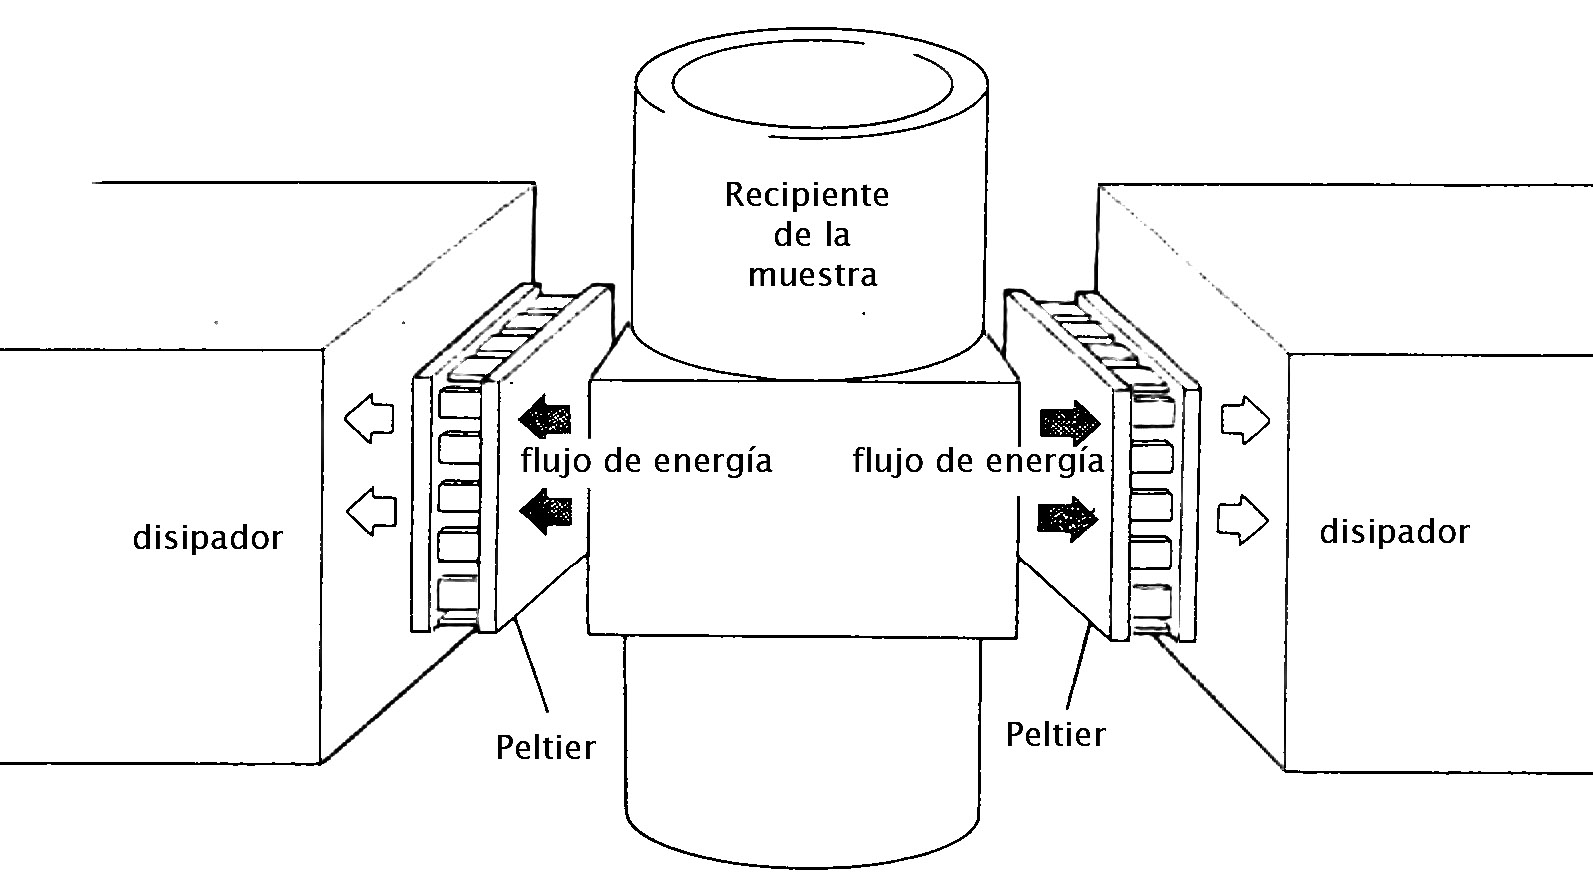
\includegraphics[width=0.59\linewidth]{../Tesis/Figures/heatFlow} & 
			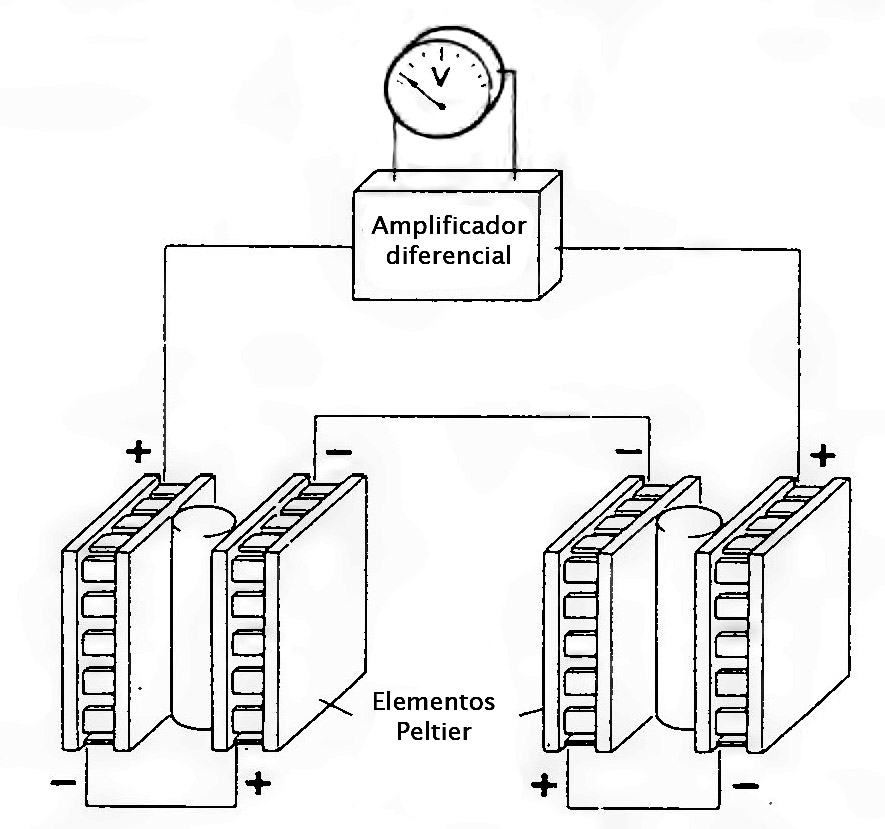
\includegraphics[width=0.39\linewidth]{../Tesis/Figures/twinMeasuring}
		\end{tabular}
		\caption{Principio de detecci\'on de la energ\'ia transferida en forma de calor para cada canal de medida del calor\'imetro, modificado de \cite{Suurkuusk}.}
	\end{figure}

	En particular, el calorímetro mide la diferencia en los flujos de energía presentados por una celda de referencia que sirve como blanco, y otra en donde se encuentra la muestra.

\section{Objetivos}
	Poner en funcionamiento el calorímetro 2277 Thermal Activity Monitor, y adicionalmente calibrar el equipo para su uso en las investigaciones activas del grupo \groupname.
	\begin{enumerate}
		\item Realizar el cableado y conexiones electrónicas pertinentes a la instalaci\'on del equipo 2277 Thermal Activity Monitor.
		\item Mantener la temperatura del ba\~no interno estable a 25 \grad{}.
		\item Realizar calibraciones eléctricas, para asegurar que las señales obtenidas tengan un equivalente en potencia.
		%			\item Determinación de la entalpía molar, energía libre de Gibbs, entropía, y constante de afinidad, de la reacci\'on de bicarbonato de potasio con \'acido clorh\'idrico como una calibración química.
		\item Determinar la entalpía de mezcla de la disolución de 1-propanol en agua.
		\item Determinar la entalpía de reacción de la neutralización del bicarbonato de potasio con el \'acido clorhídrico.
		\item Obtener el factor calorimétrico del calorímetro.
	\end{enumerate}

\section{Instalaci\'on del calor\'imetro}
	El primer paso consistió en ajustar los voltajes de operación del calorímetro de 225 VAC a 110 VAC, junto con el cambio de dos fusibles con capacidad para el doble de corriente.
	
	\begin{figure}
		\centering
		\begin{tabular}{cccc}
			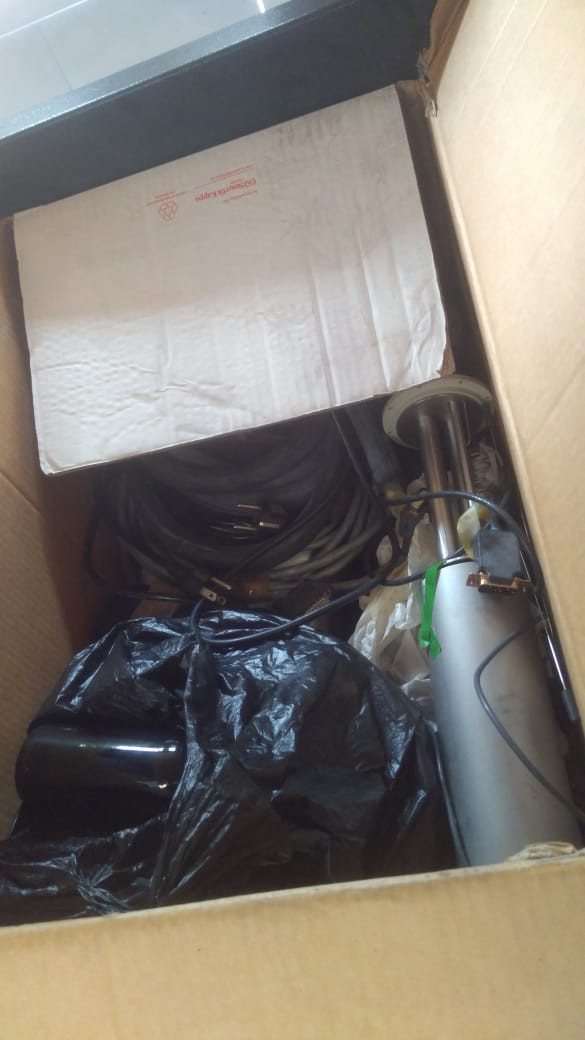
\includegraphics[width=0.2\linewidth]{../Tesis/Figures/process/box1} & 
			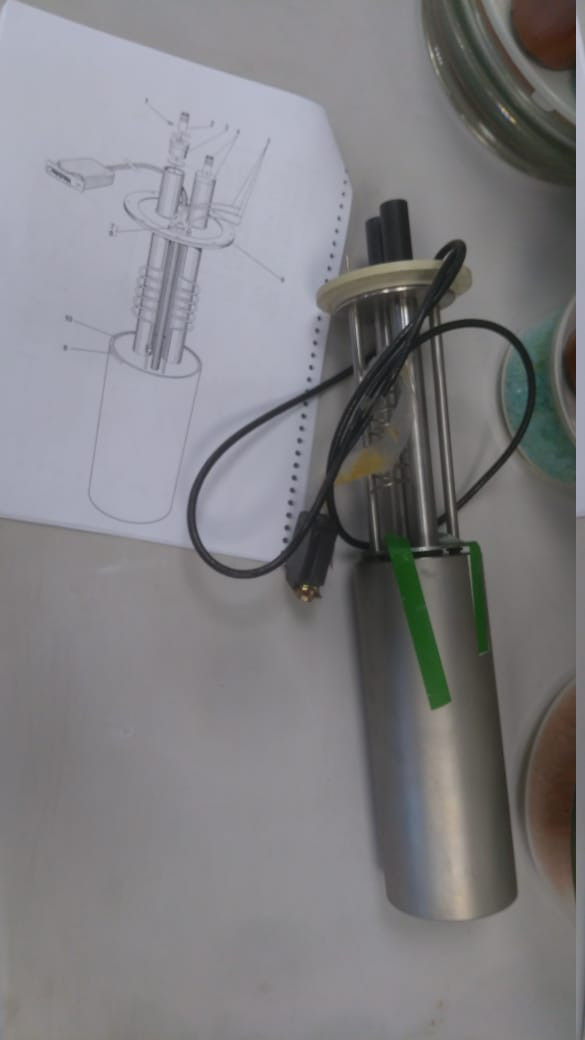
\includegraphics[width=0.2\linewidth]{../Tesis/Figures/process/holder} &
			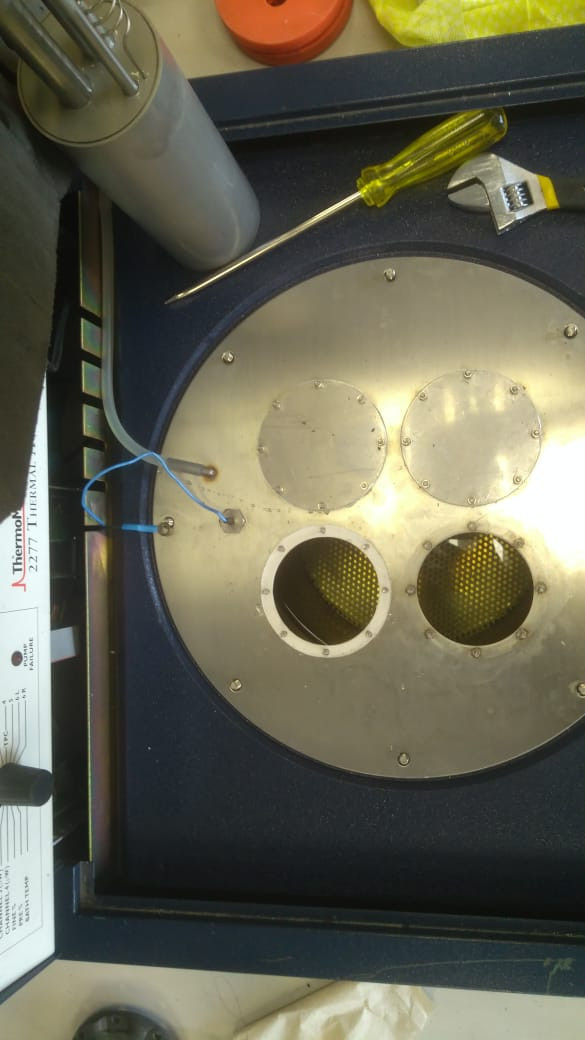
\includegraphics[width=0.2\linewidth]{../Tesis/Figures/process/p1} & 
			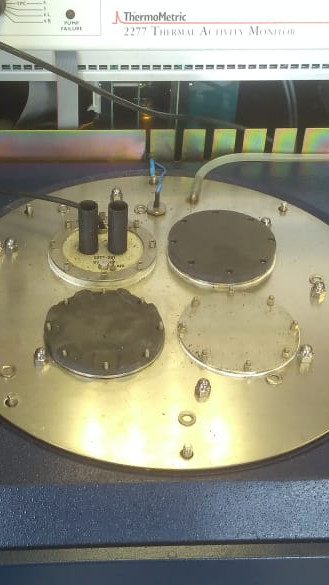
\includegraphics[width=0.2\linewidth]{../Tesis/Figures/process/p2} \\ 
			& 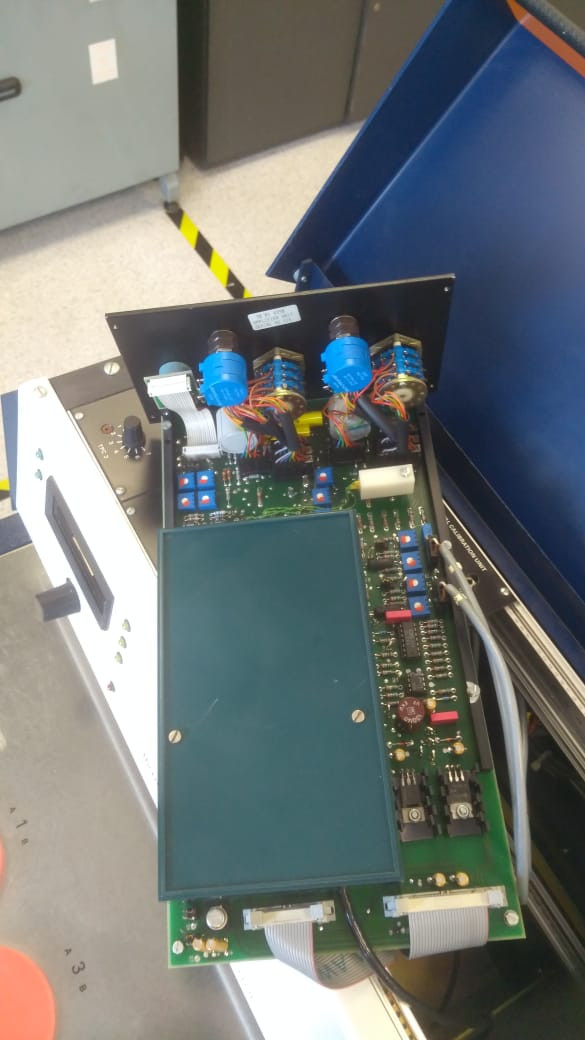
\includegraphics[width=0.2\linewidth]{../Tesis/Figures/process/p3} & 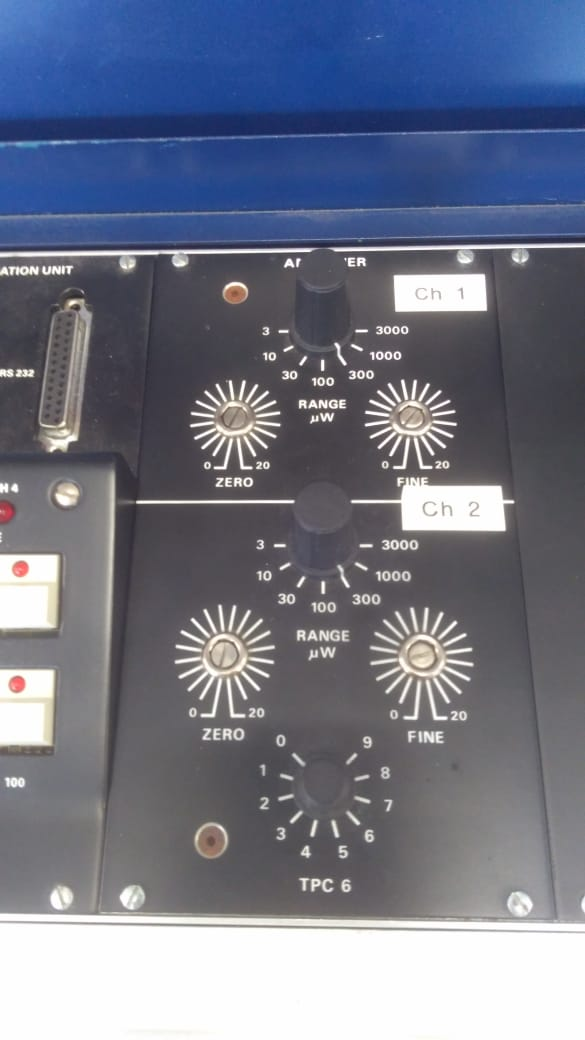
\includegraphics[width=0.2\linewidth]{../Tesis/Figures/process/p4} \\
		\end{tabular}
		\caption{Proceso de instalación de un cilindro de medición.}
	\end{figure}
	
	Posteriormente, se instaló un cilindro de medición y se estableció la comunicación con un computador reemplazando el protocolo RS232 por USB usando el programa Digitam 4. El circuito del motor del agitador de la celda se modificó para operar con 5 V, los cuales se obtienen usando un puerto USB. Los experimentos de titulaci\'on calorim\'etrica requieren de constante agitaci\'on sobre la celda, para conocer el efecto de este sobre las lecturas de potencia, se realizaron 6 ciclos de conexi\'on y desconexi\'on del agitador, obteniendo los siguientes resultados: $2.1\pm0.2$ y $-1.9\pm0.2$ $\mu$W, respectivamente.
	\begin{figure}[h]
		\centering
		\begin{tabular}{cc}
			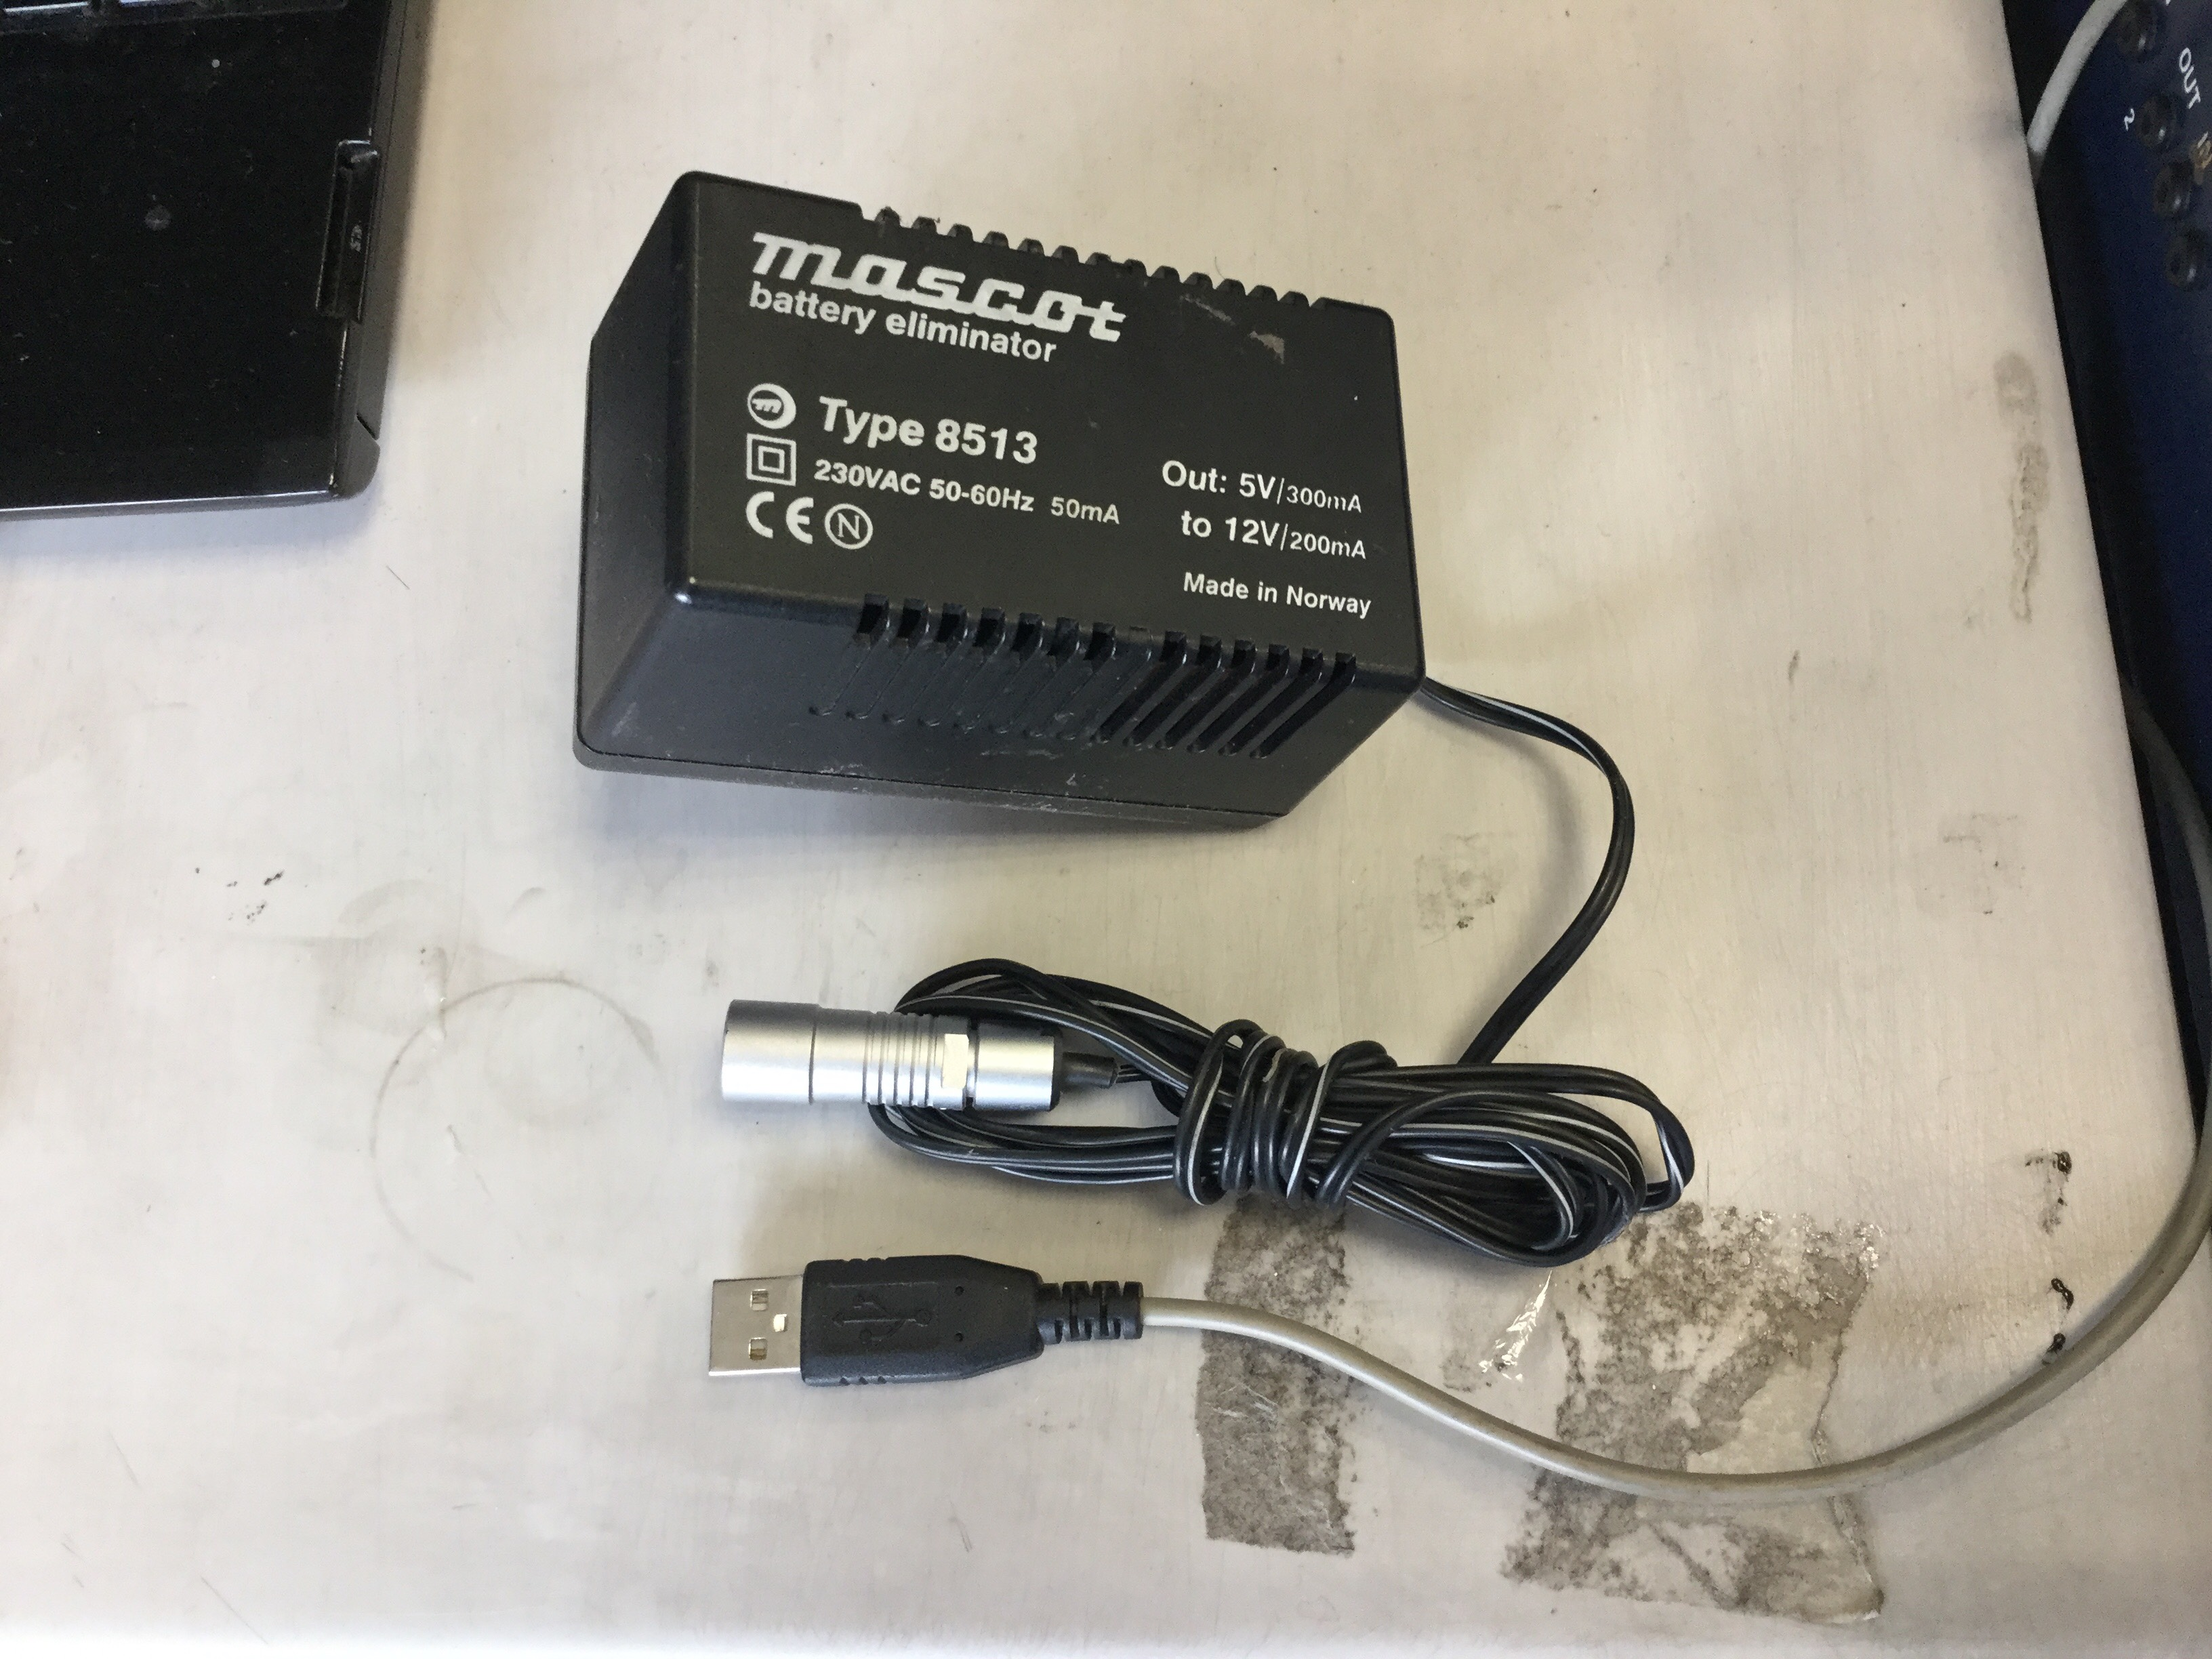
\includegraphics[width=0.3\linewidth]{../Tesis/Figures/motorCircuit}
			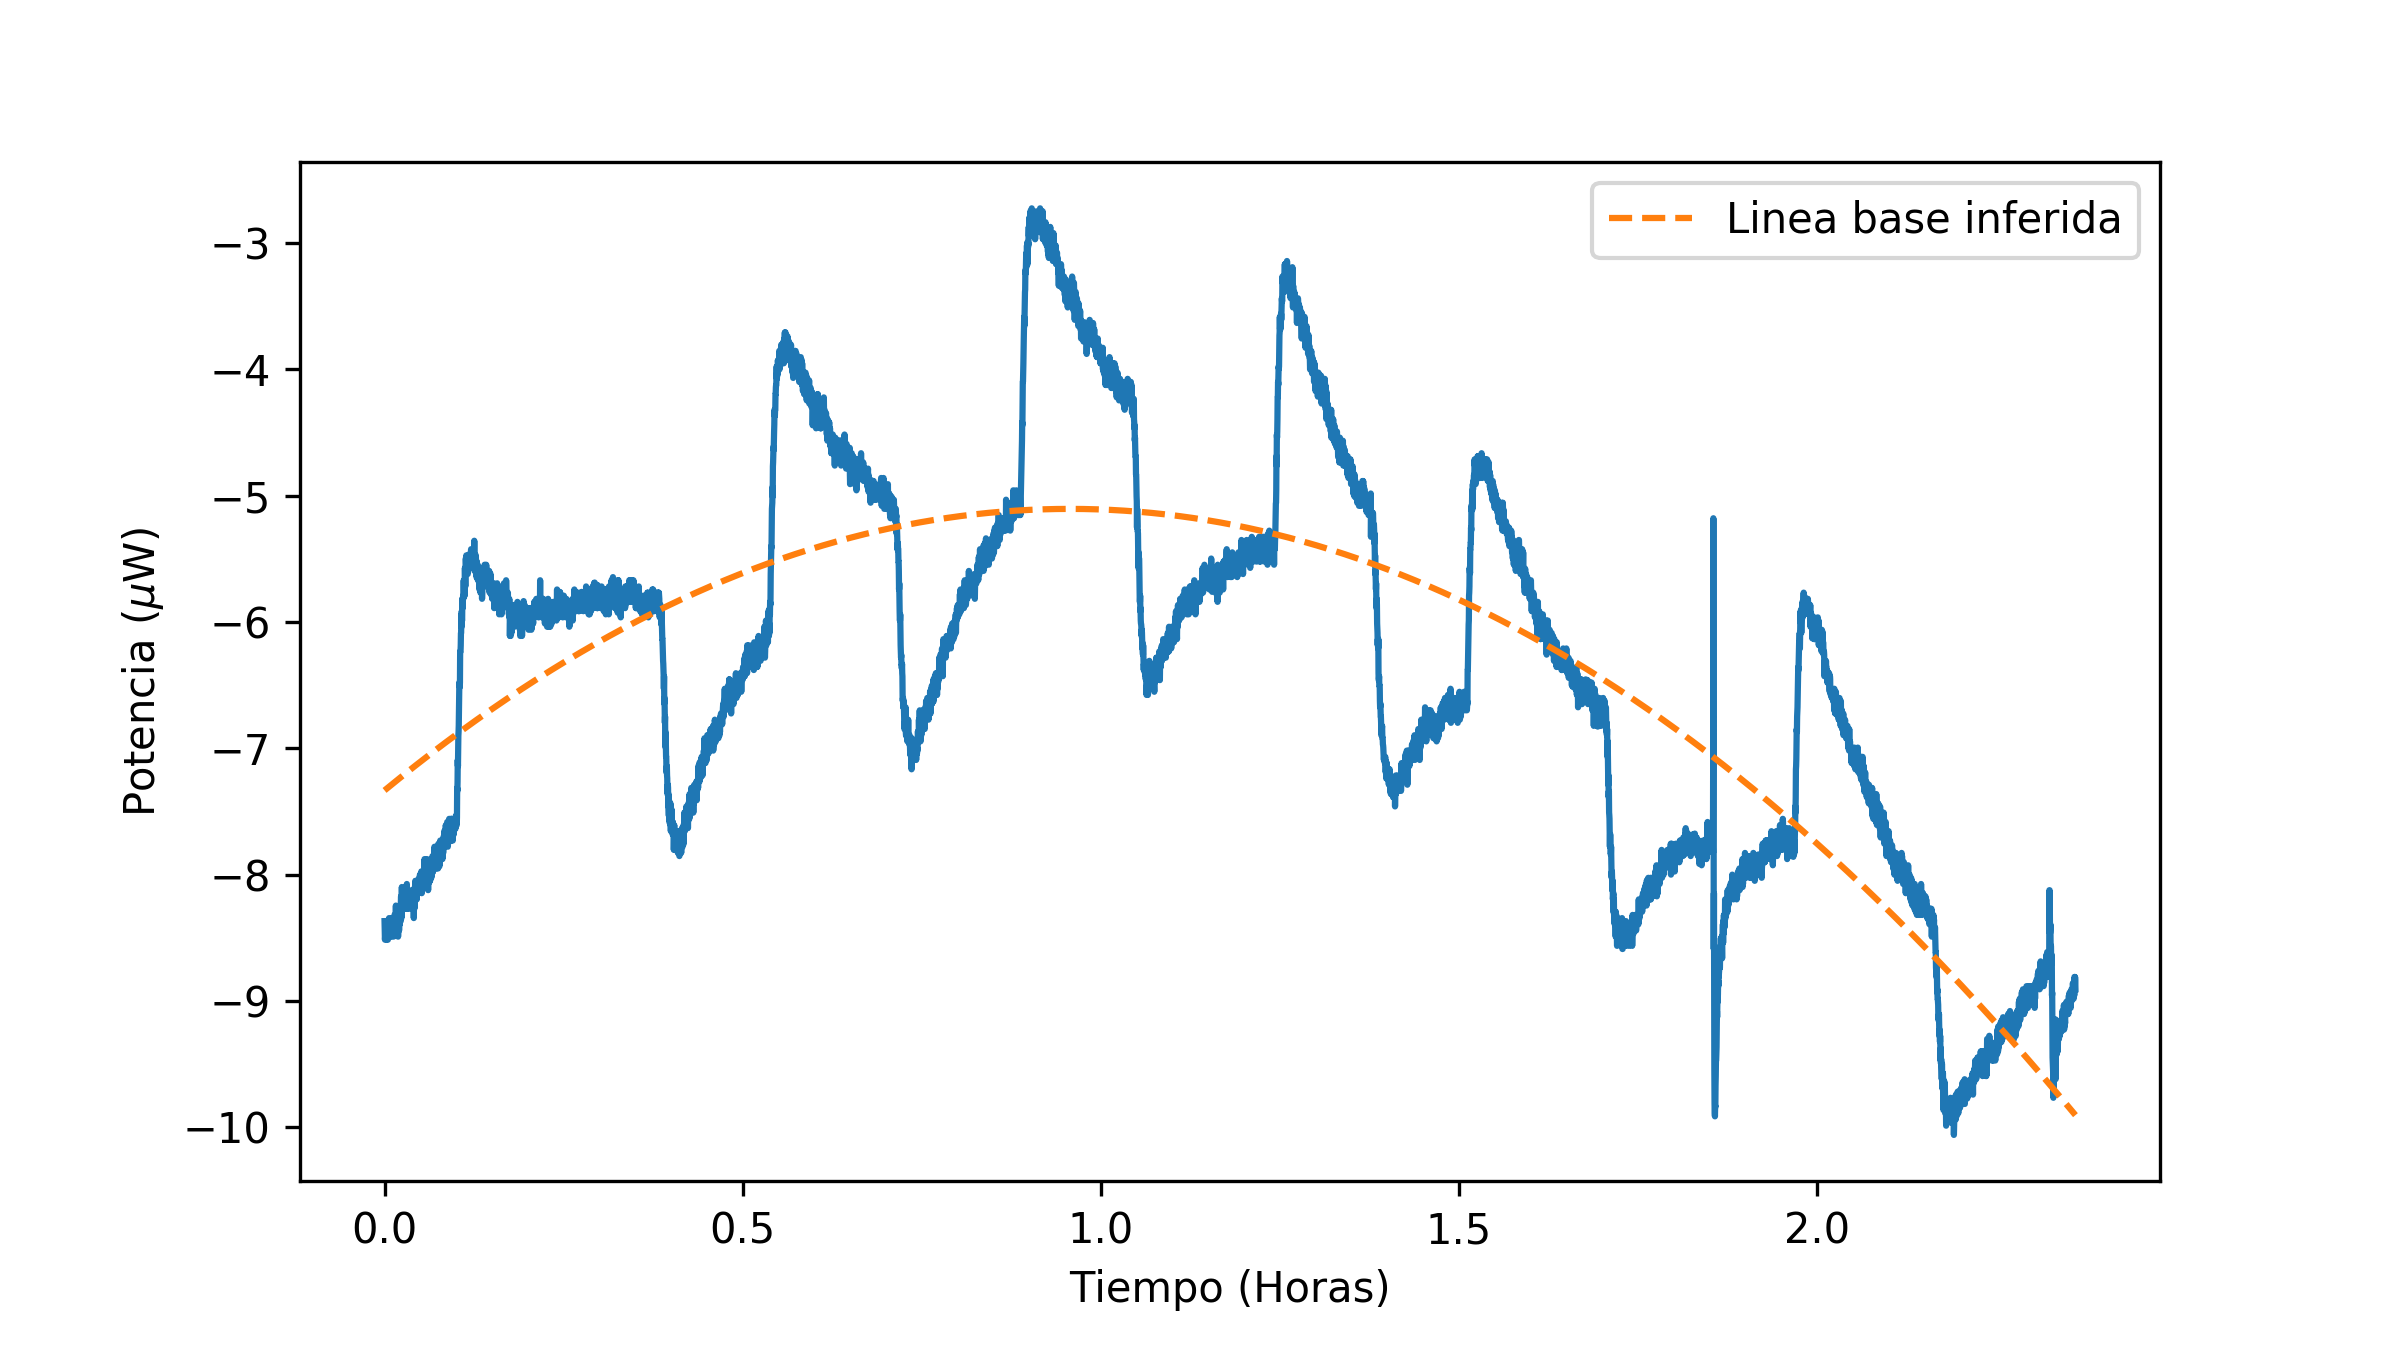
\includegraphics[width=0.7\linewidth]{../Data/Baselines/motor}
		\end{tabular}
		\caption{Comparación de los sistemas de alimentación del motor, junto con los resultados de los ciclos de conexión y desconexión del agitador.}
	\end{figure}

\section{Control de la temperatura}
	La temperatura del baño interno del calorímetro se controla usando cuatro resistencias de década, junto con la temperatura de un baño externo. Encontrar la combinación de estos parámetros que permitiera estabilizar el calorímetro a 25 \grad{} requirió de un sistema de monitoreo de la temperatura en tiempo real. Este sistema fue construído usando un microcontrolador ATtiny13, y tres sensores LM35.

	\begin{figure}[h]
		\centering
		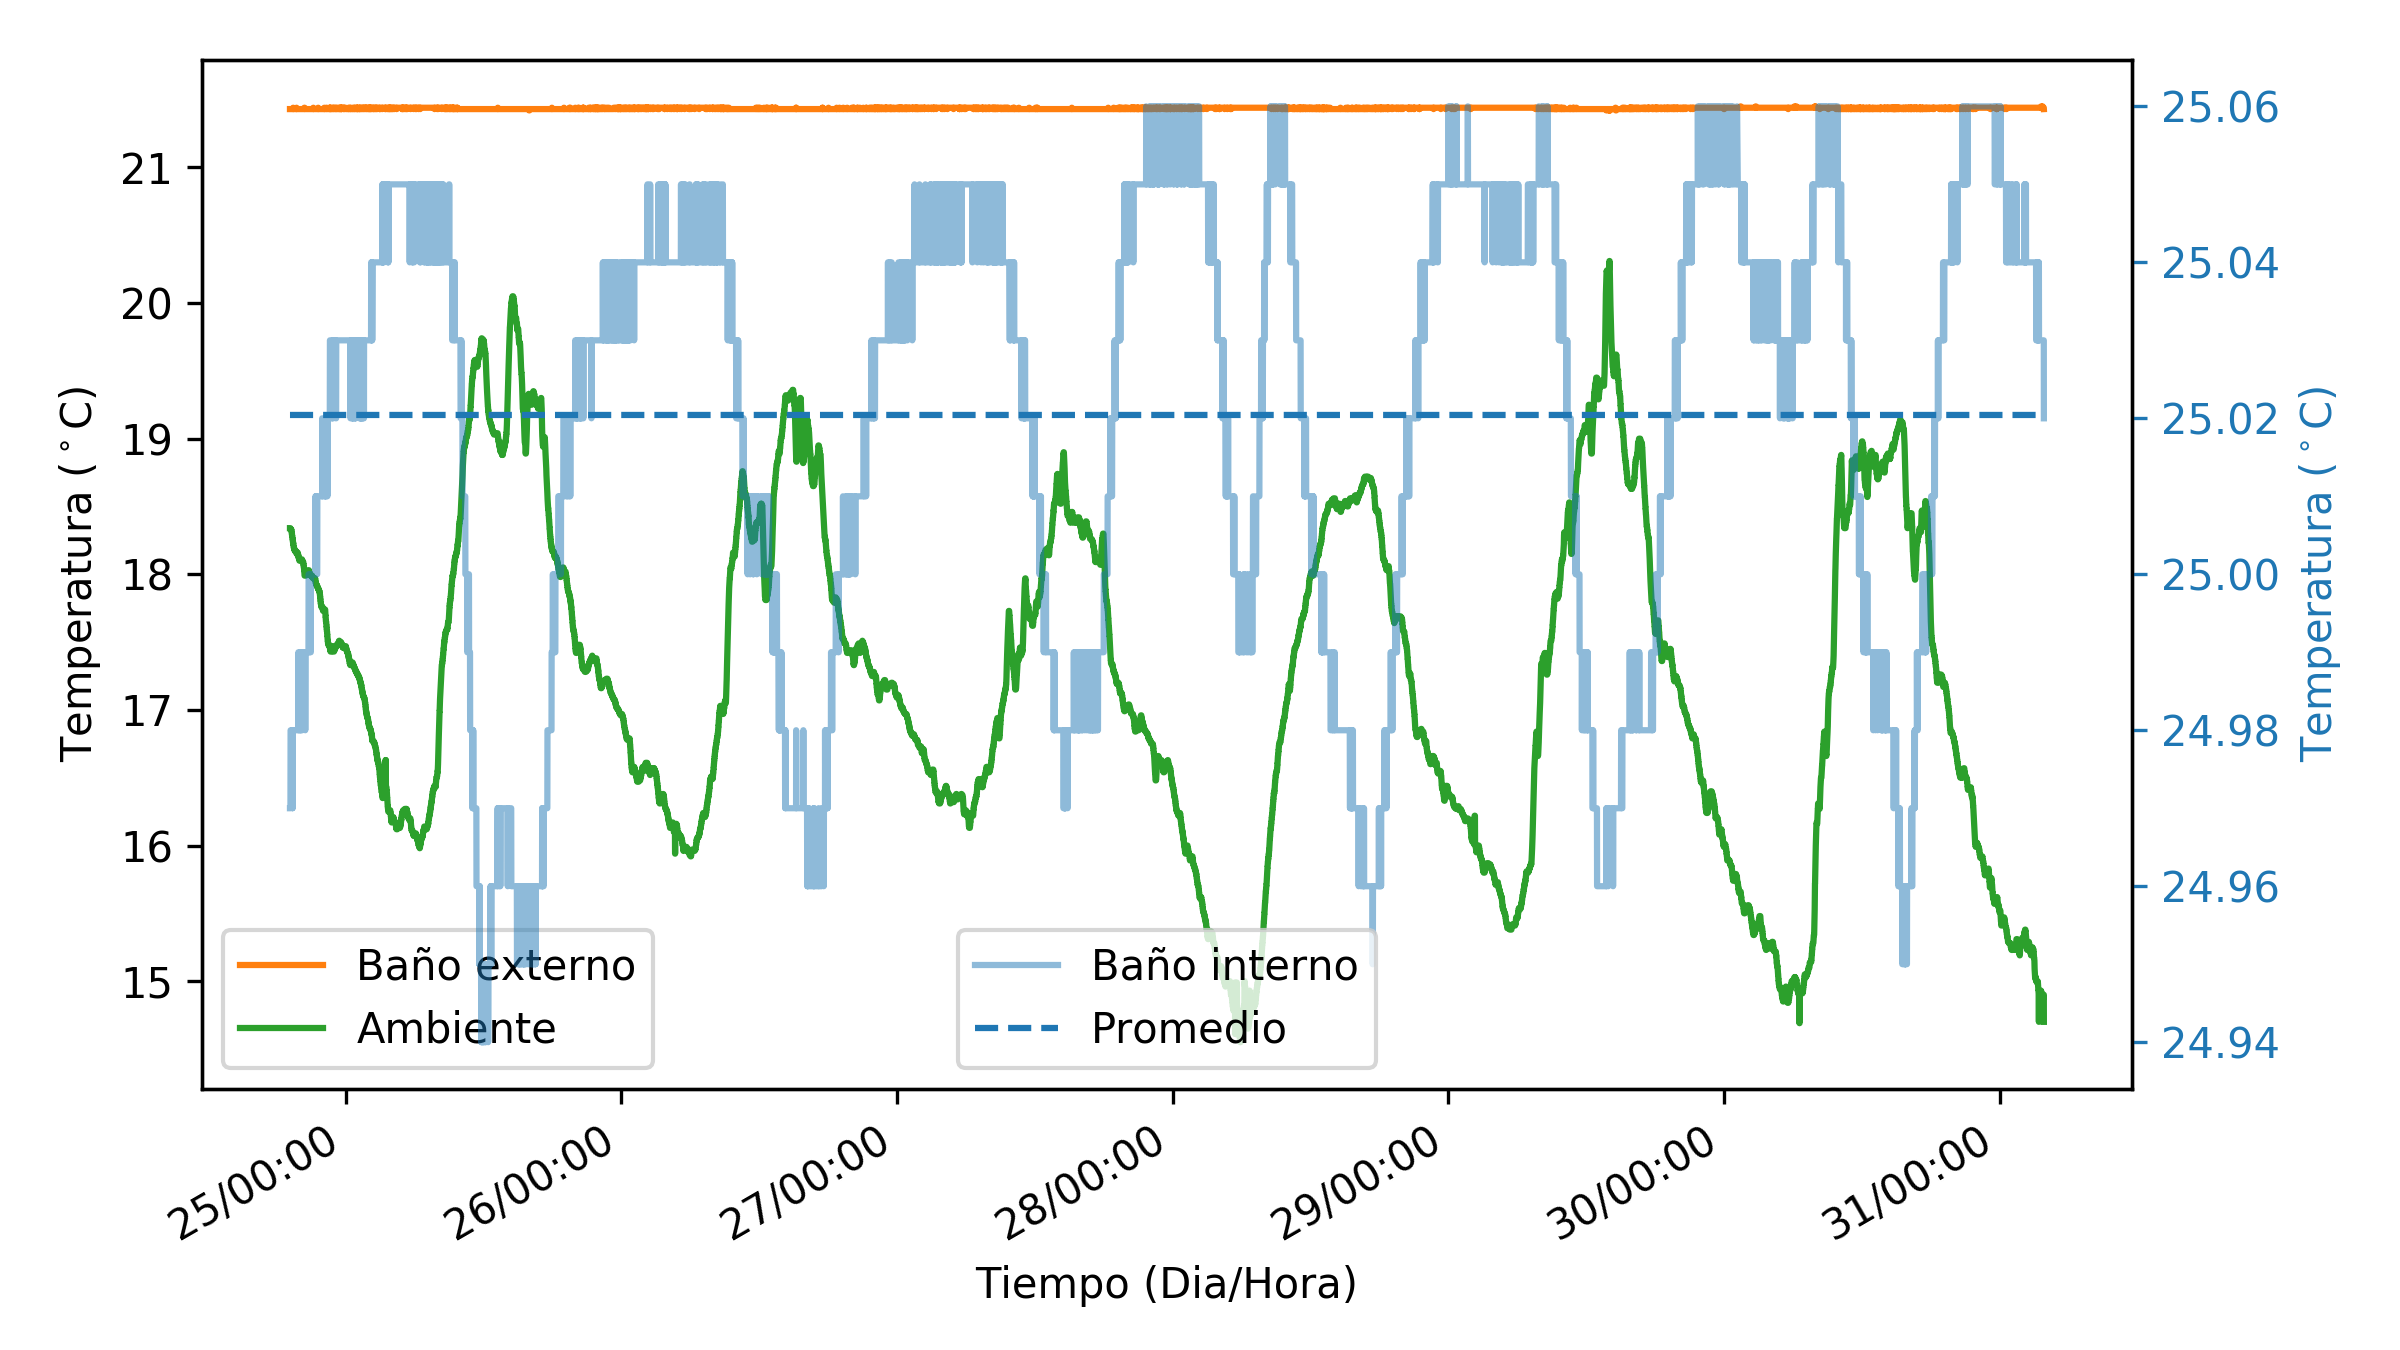
\includegraphics[width=\figwidth]{../Data/TemperatureStability/temperatureStability}
		\caption{Efecto de la temperatura ambiente sobre la temperatura del baño interno a $25.02\pm0.03$ \grad{}. La escala para las curvas azules se encuentra al lado derecho.}
	\end{figure}
	
	La temperatura interna del calorímetro se encuentra correlacionada con la temperatura ambiente, los máximos de temperatura interna ocurren en los mínimos de temperatura ambiente. Esta correlaci\'on fue cuantificada con un coeficiente de correlaci\'on de -0.77.
	
%	Esta correlaci\'on es cuantificada con el coeficiente de correlaci\'on entre los datos $i, j$ se calcula usando la entrada $i,j$ de la matriz de covarianza asociada \cite{landau2008survey}.
%	\begin{equation}
%		c = \dfrac{\text{cov}(i, j)}{\sigma_i\sigma_j} = \dfrac{E((\mathbf{x_i} - 	\bar{x}_i)(\mathbf{x_j} - \bar{x}_j))}{\sigma_i\sigma_j}
%	\end{equation}
%	
%	Donde $E$ es la funci\'on que retorna el valor esperado de un vector ($\bar{x}_i = E(\mathbf{x_i})$ promedio), se obtiene $c = -0.77$. 

\section{Calibraci\'on El\'ectrica}
	Con el objetivo de asegurar que la información registrada por el calorímetro corresponde con un valor específico de potencia, es necesario realizar una calibración eléctrica.
	\begin{figure}[h]
		\centering
		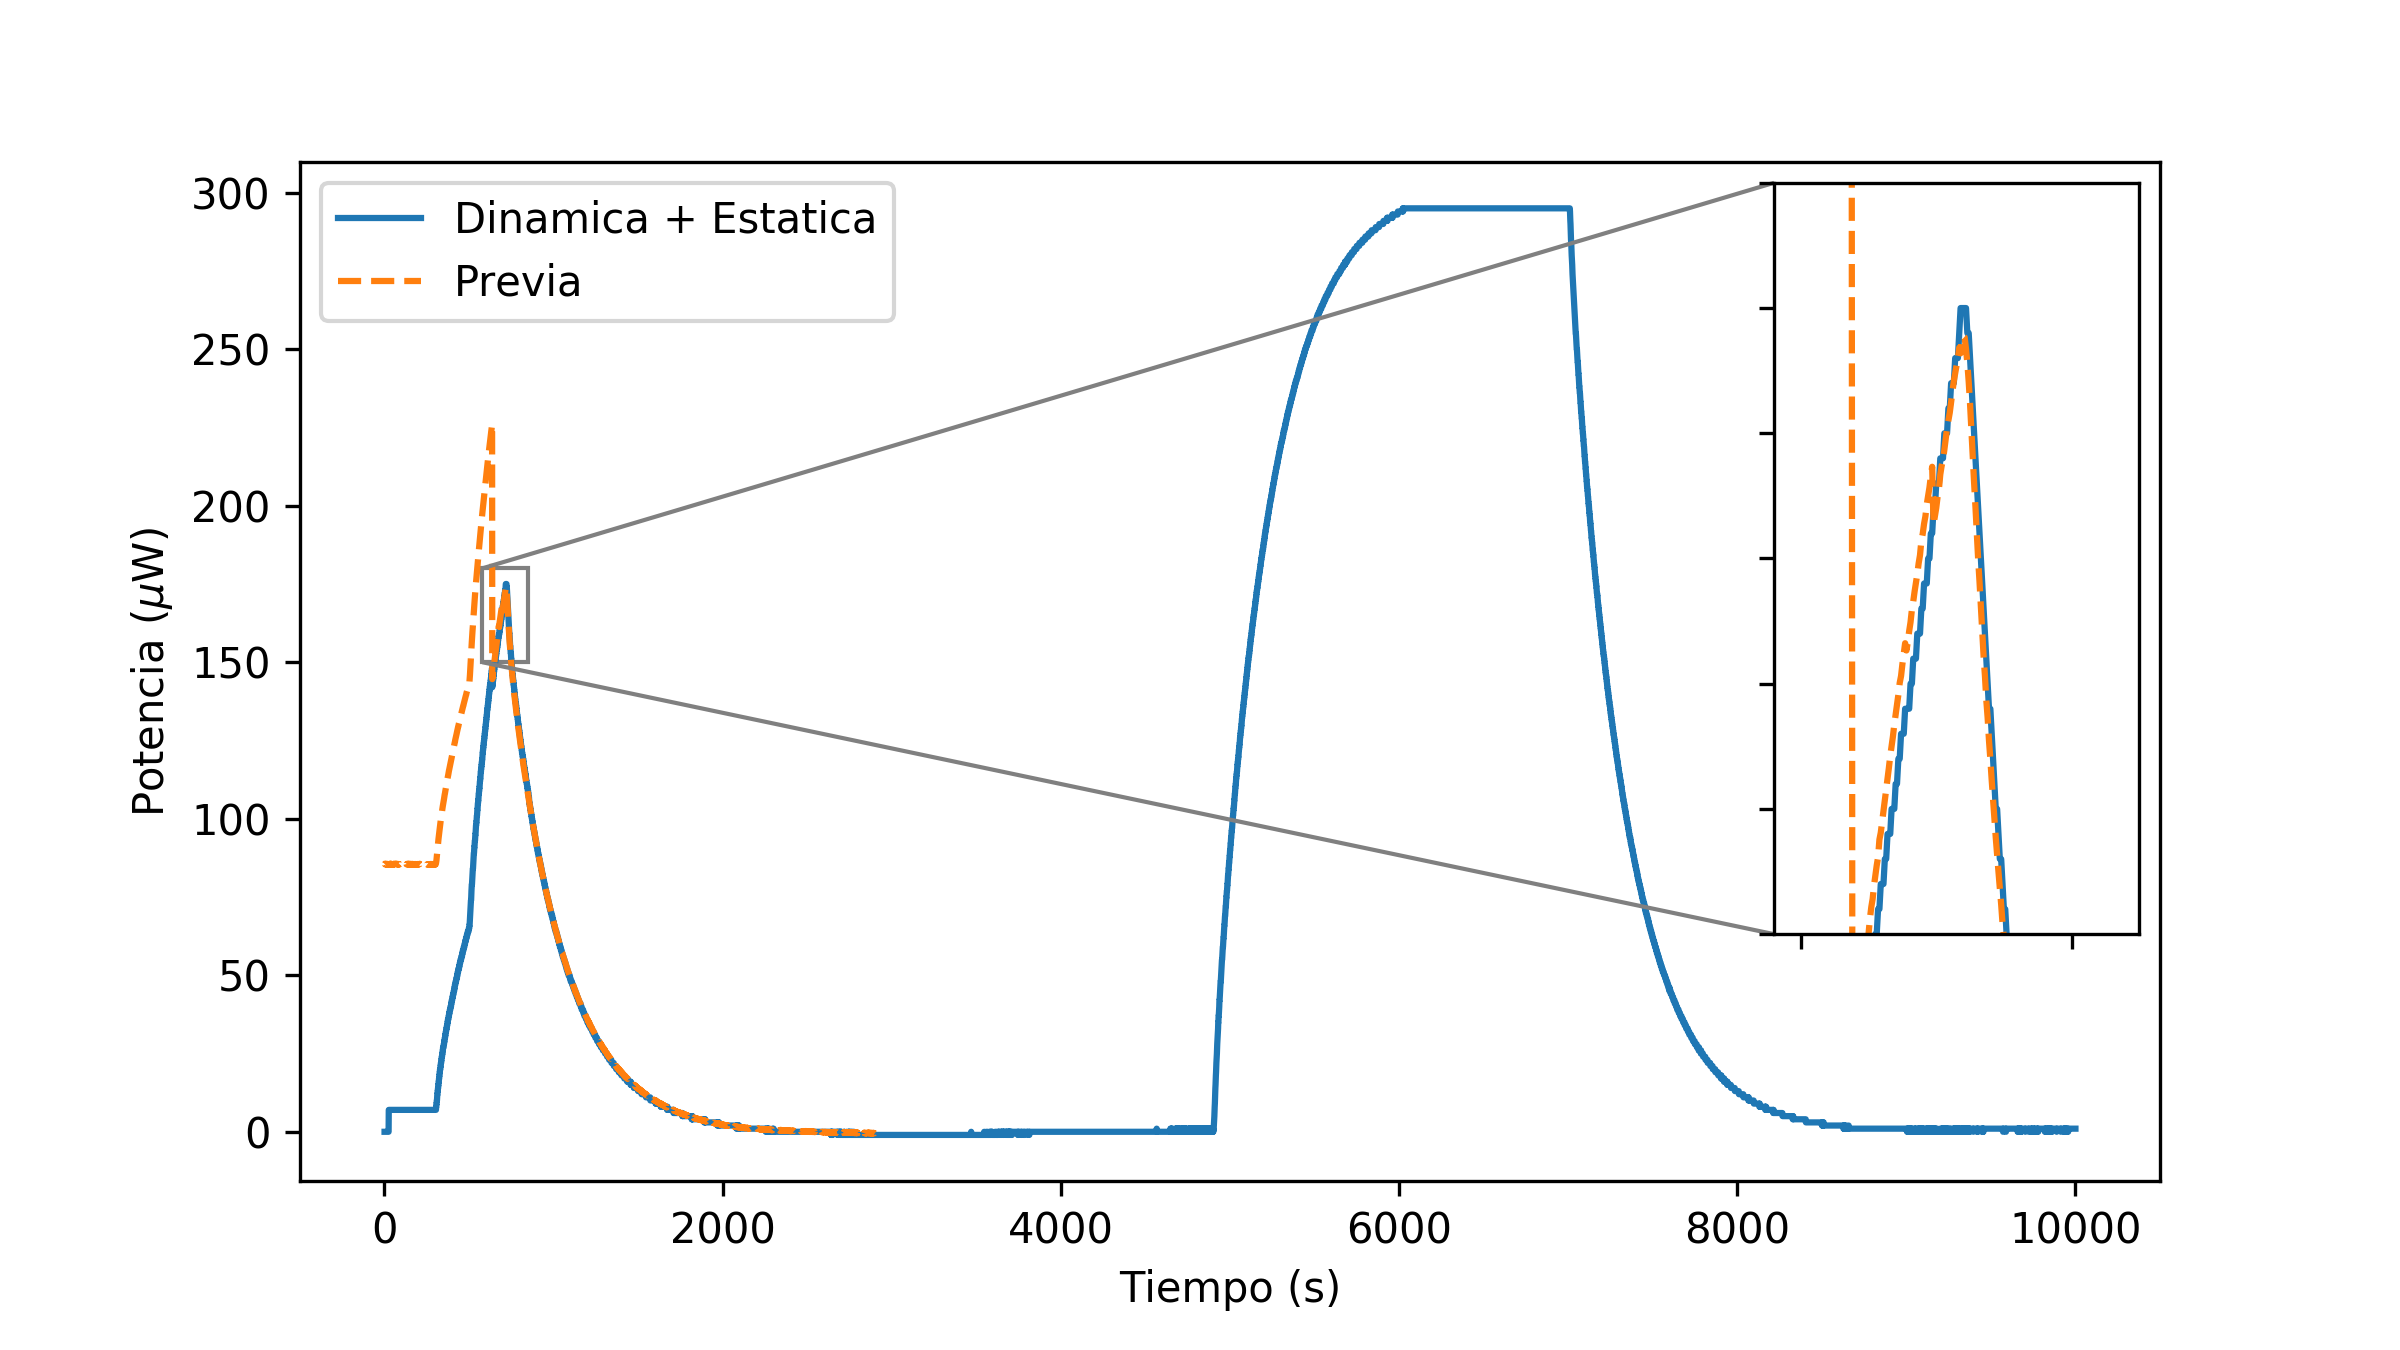
\includegraphics[width=\figwidth]{../Data/ElectricalCalibrations/Both}
		\caption{Calibraciones dinámica y estática que muestran el correcto funcionamiento del calorímetro.}
	\end{figure}

	Existen dos tipos de calibraciones, en la primera se modifica el cero y ganancia del calorímetro en el circuito análogo, mientras que en la segunda los valores se ajustan por software. 

\section{Calibraci\'on Qu\'imica}
	La calibraci\'on qu\'imica consiste en contrastar las propiedades termodin\'amicas de un sistema qu\'imico obtenidas usando el calor\'imetro con aquellas reportadas en la literatura. 
	\begin{figure}[h]
		\centering
		\begin{tabular}{cc}
			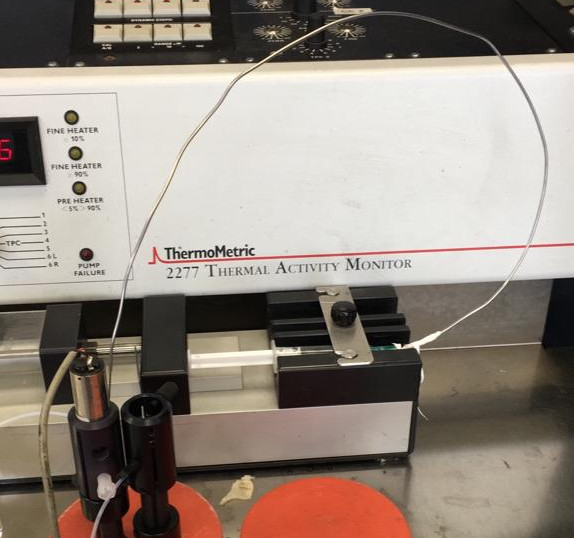
\includegraphics[width=0.4\linewidth]{../Tesis/Figures/sistemaInyeccion} & 
			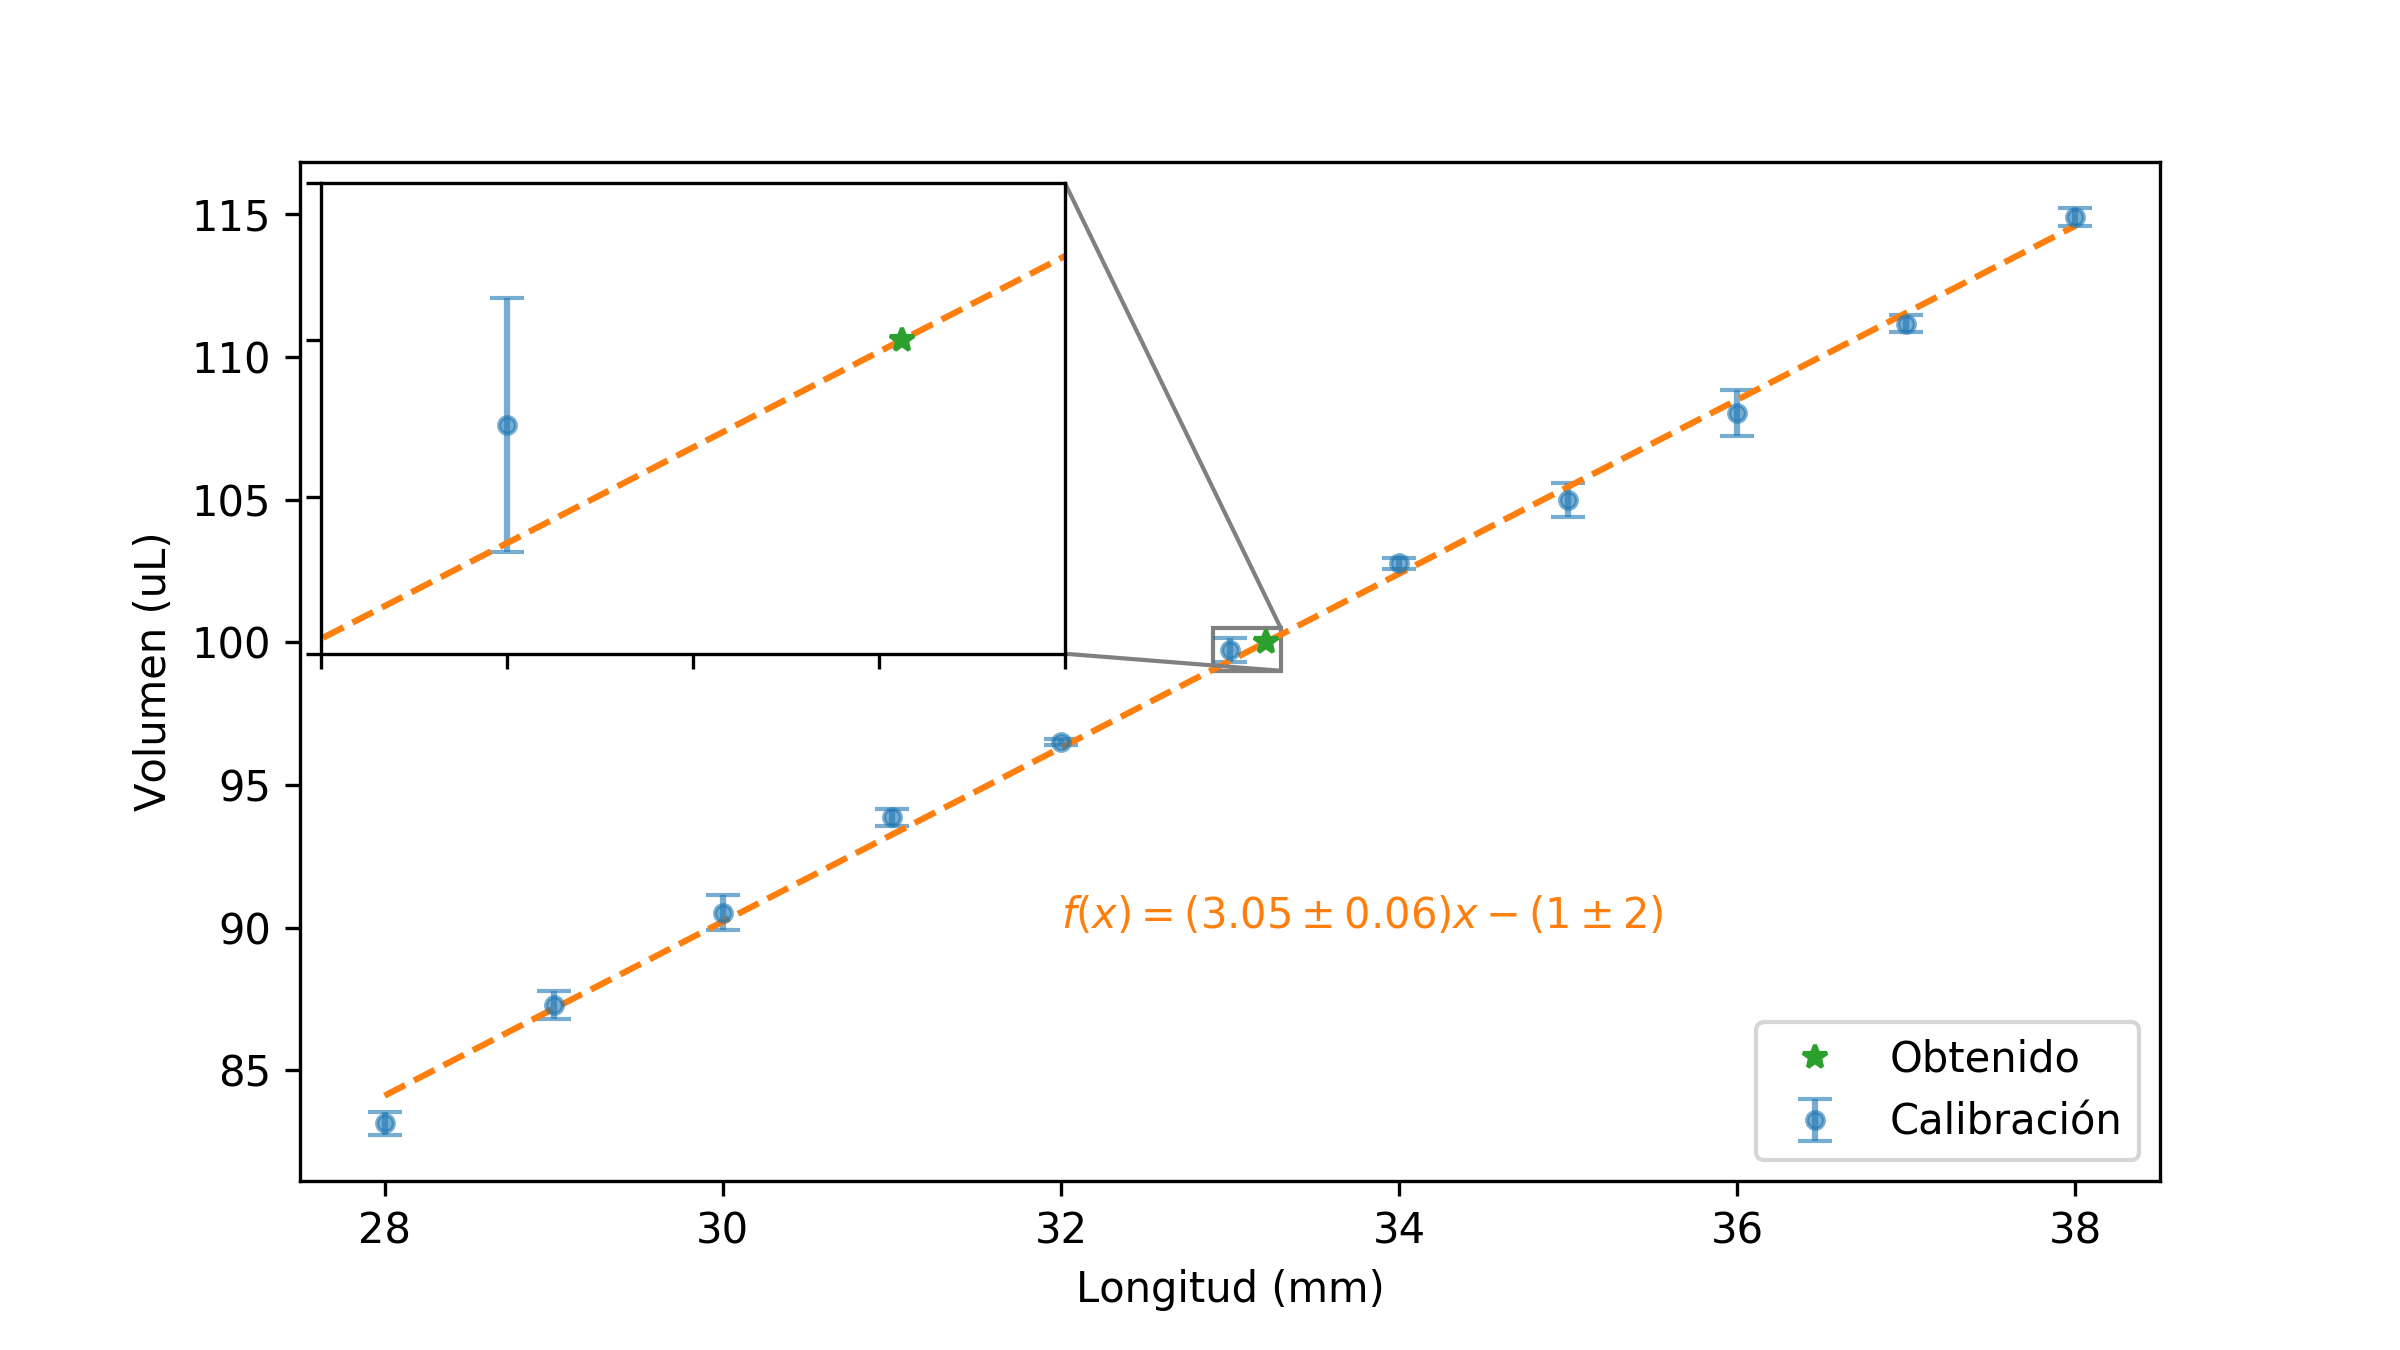
\includegraphics[width=0.6\linewidth]{../Data/Syringe/syringe_cal.png}
		\end{tabular}
		\caption{Sistema de inyección construido como alternativa al uso de cánulas, junto con la calibración de la jeringa.}
	\end{figure}

	Dos sistemas qu\'imicos fueron usados para la realizaci\'on de la calibraci\'on qu\'imica: la disoluci\'on de 1-propanol en agua y la reacci\'on del \'acido clorhídrico con bicarbonato de potasio \cite{demarse2011calibration, adao2012chemical, nanoitc}. La energía liberada por inyección se calcula al integrar la potencia registrada, la cual, al considerar la primera ley de la termodinámica $U = Q-\int pdV$ y la entalpía $\Delta H = Q + V\Delta p$ a presiones constantes, da lugar a:
	\begin{equation}
		\int\limits_t^{t+\Delta t_\text{iny}} Pdt = Q_\text{iny} = -\Delta_\text{iny}H
	\end{equation}
	
	Para obtener la soluci\'on de 1-propanol al 2.96 \% (p/p) se mezclaron 1.0290 g de 1-propanol en 33.6457 g de agua tipo 1. Con esta soluci\'on, se realizaron dos experimentos con una \'unica inyecci\'on de 1.382 mL de 1-propanol a 2.5 mL de agua.
	
	\begin{figure}[h]
		\centering
		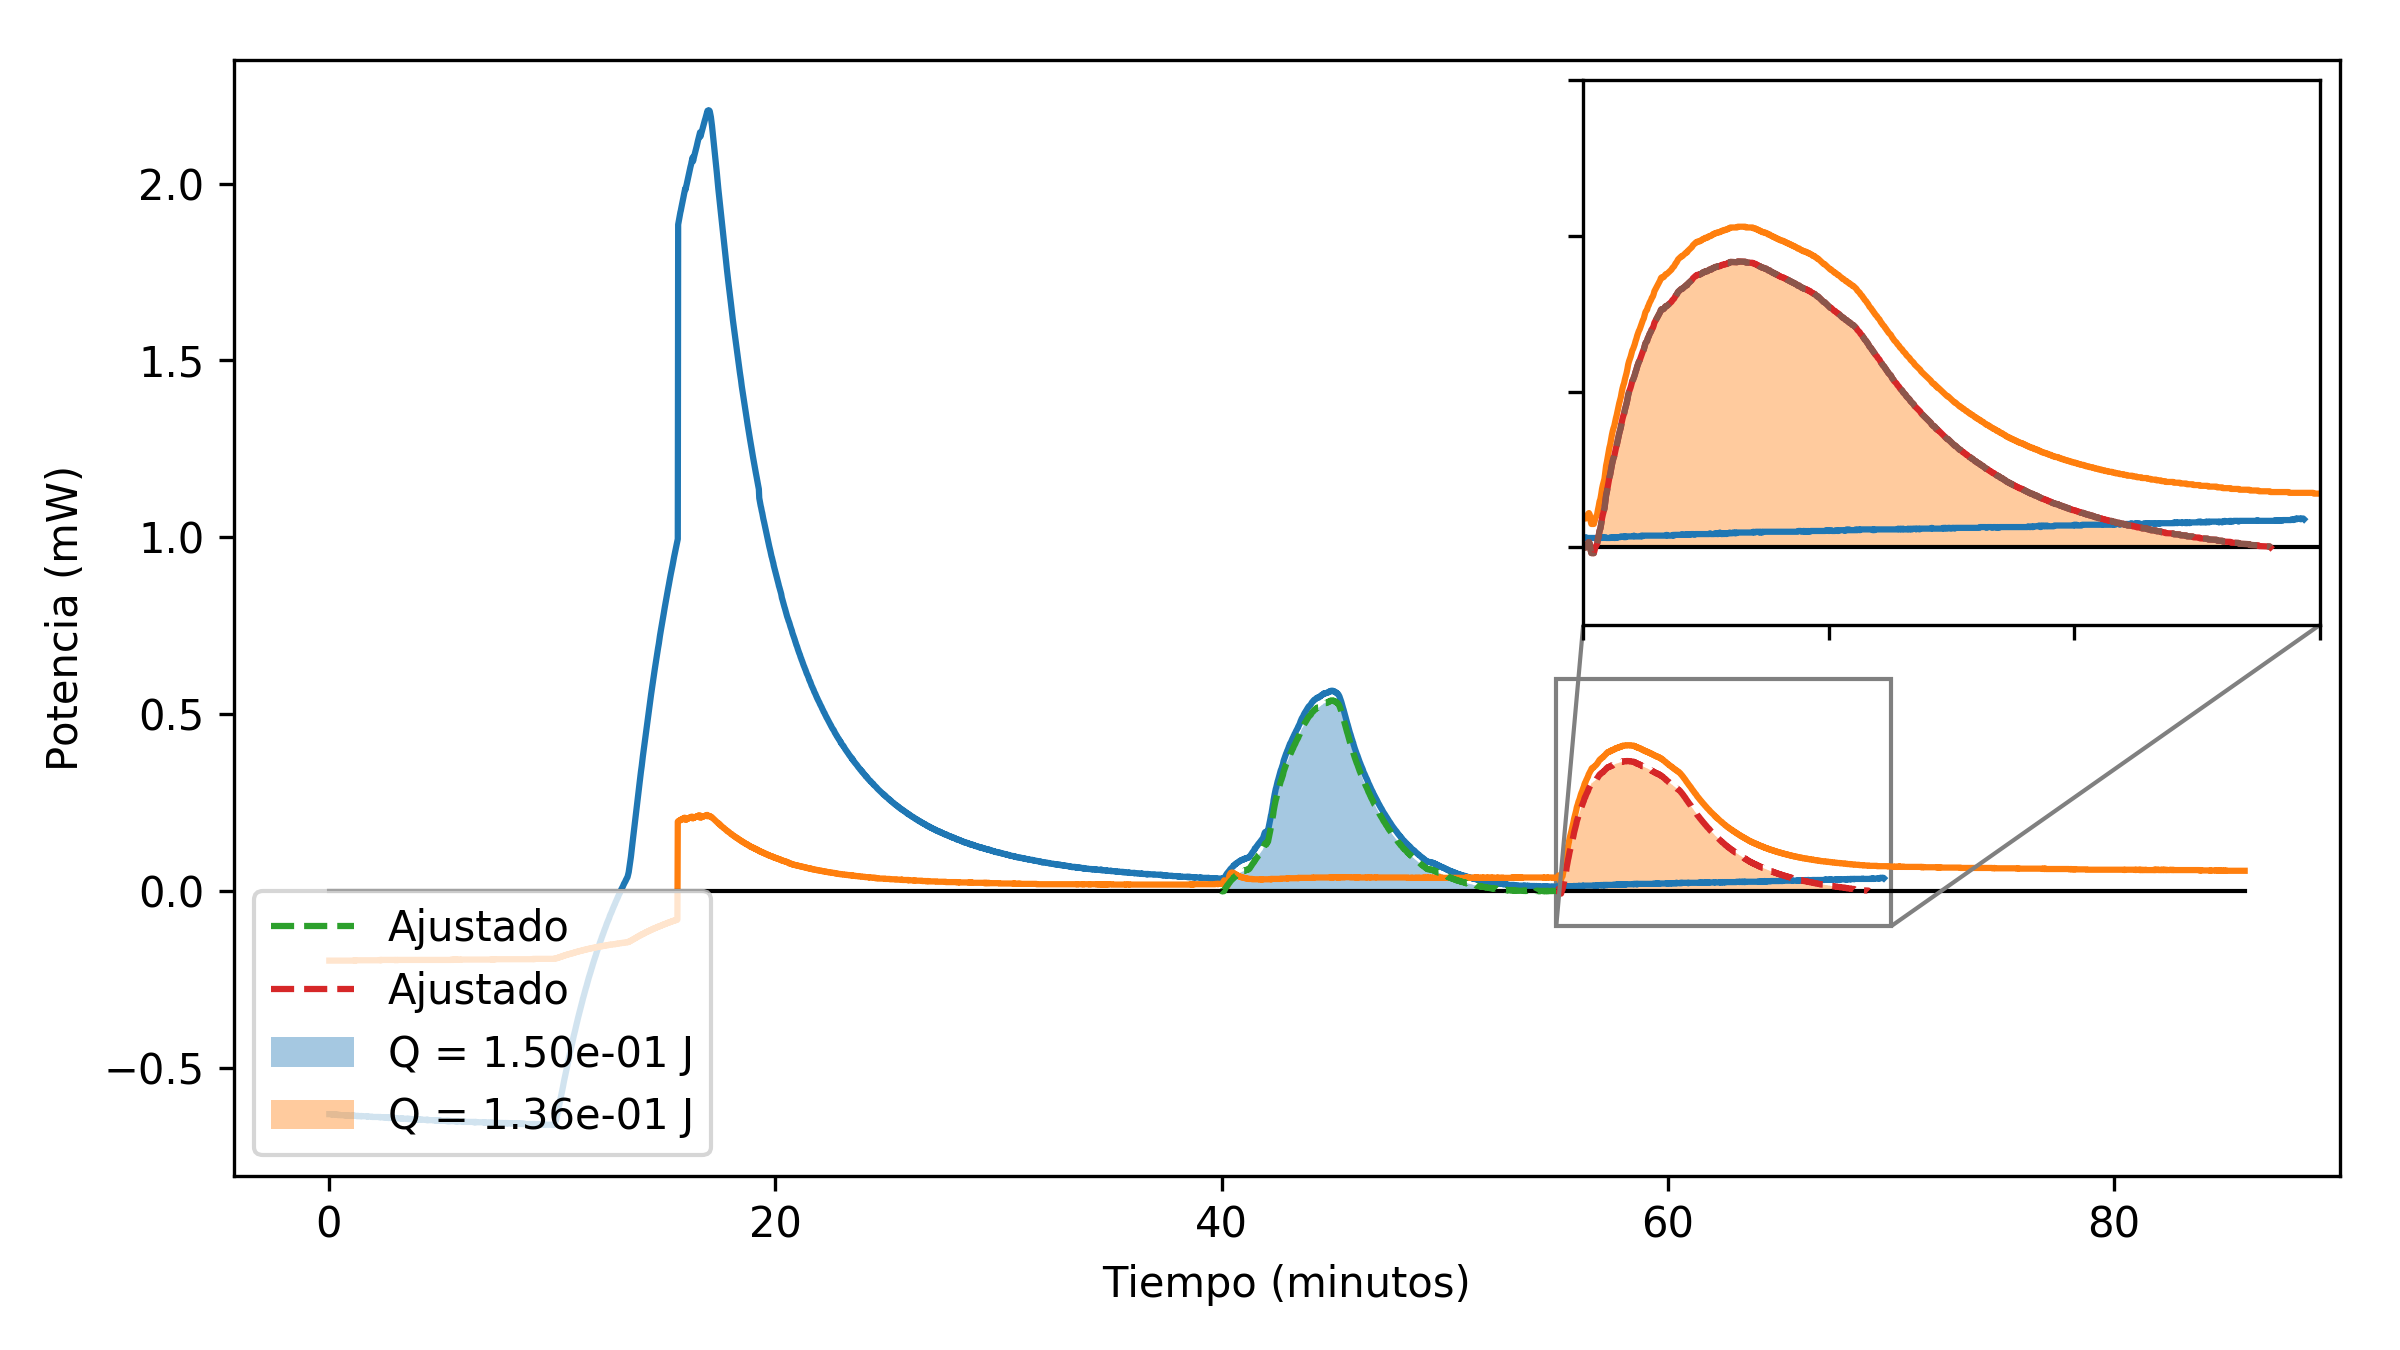
\includegraphics[width=\figwidth]{../Data/ChemicalCalibrations/singlePropanol}
		\caption{Resultados obtenidos para la mezcla de 1-propanol 2.96 \% (p/p) con agua, en una \'unica inyecci\'on, $\Delta H$ = -221 y -201 kJ/mol.}
	\end{figure}

	Un tercer experimento se llev\'o a cabo realizando 27 inyecciones de 51.185 $\mu$L con tiempos de espera entre cada una de ellas, de 5 minutos.
	
	\begin{figure}[h]
		\centering
		\begin{tabular}{cc}
			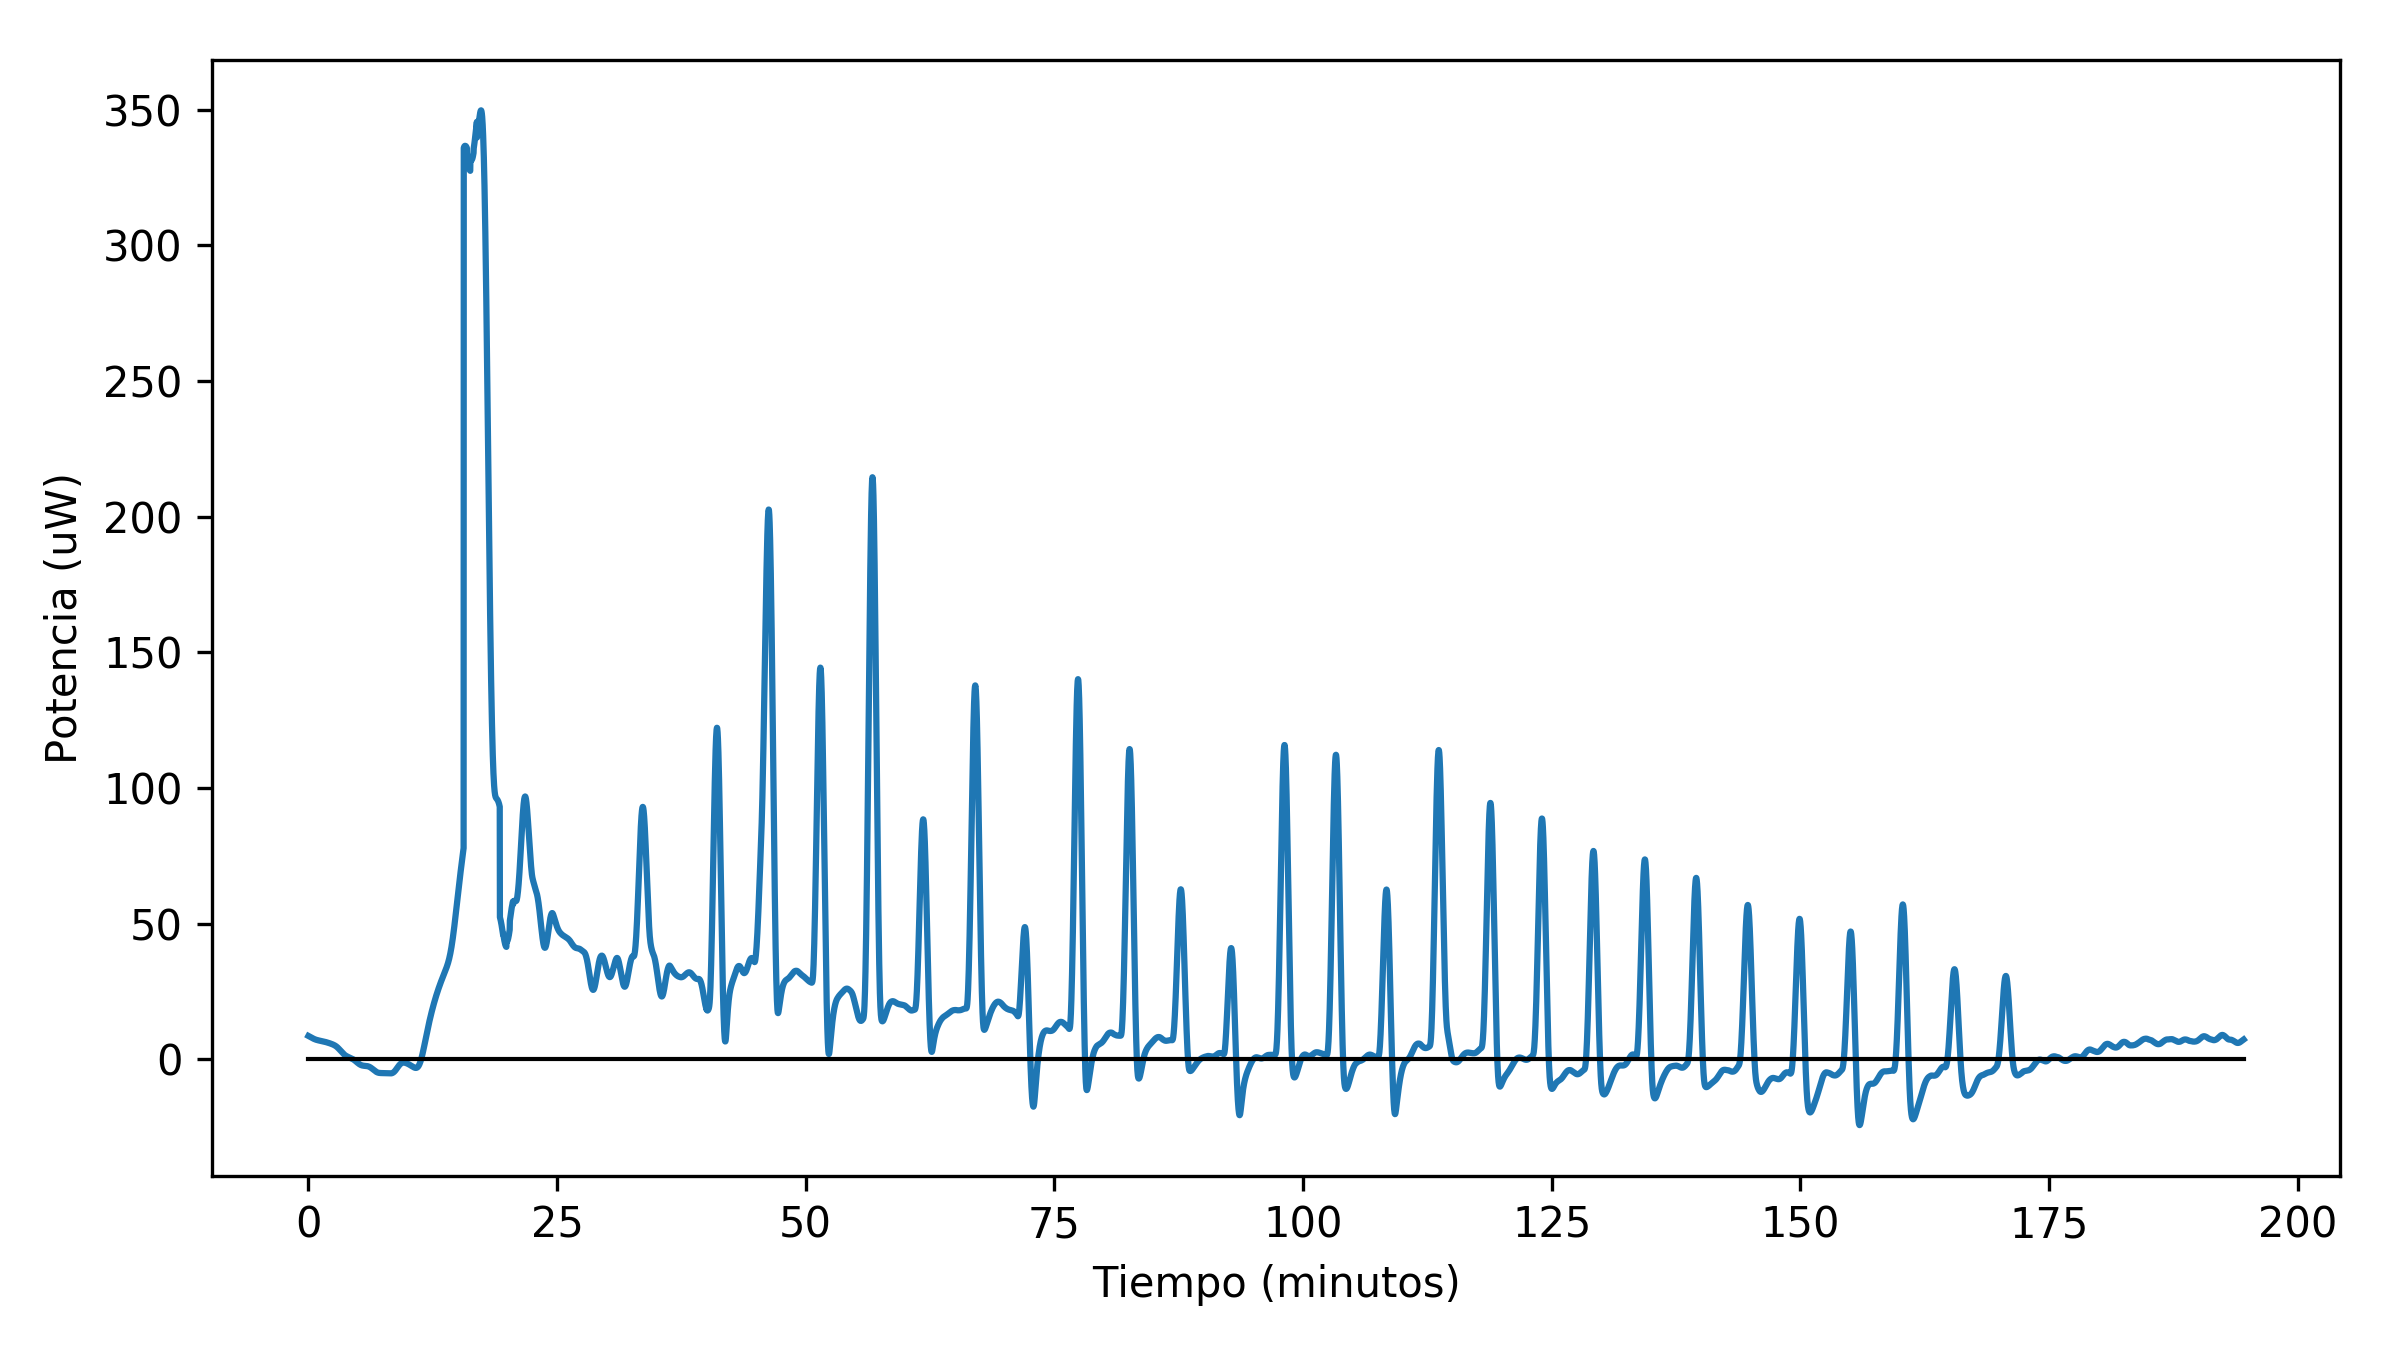
\includegraphics[width=0.47\linewidth]{../Data/ChemicalCalibrations/multiple}
			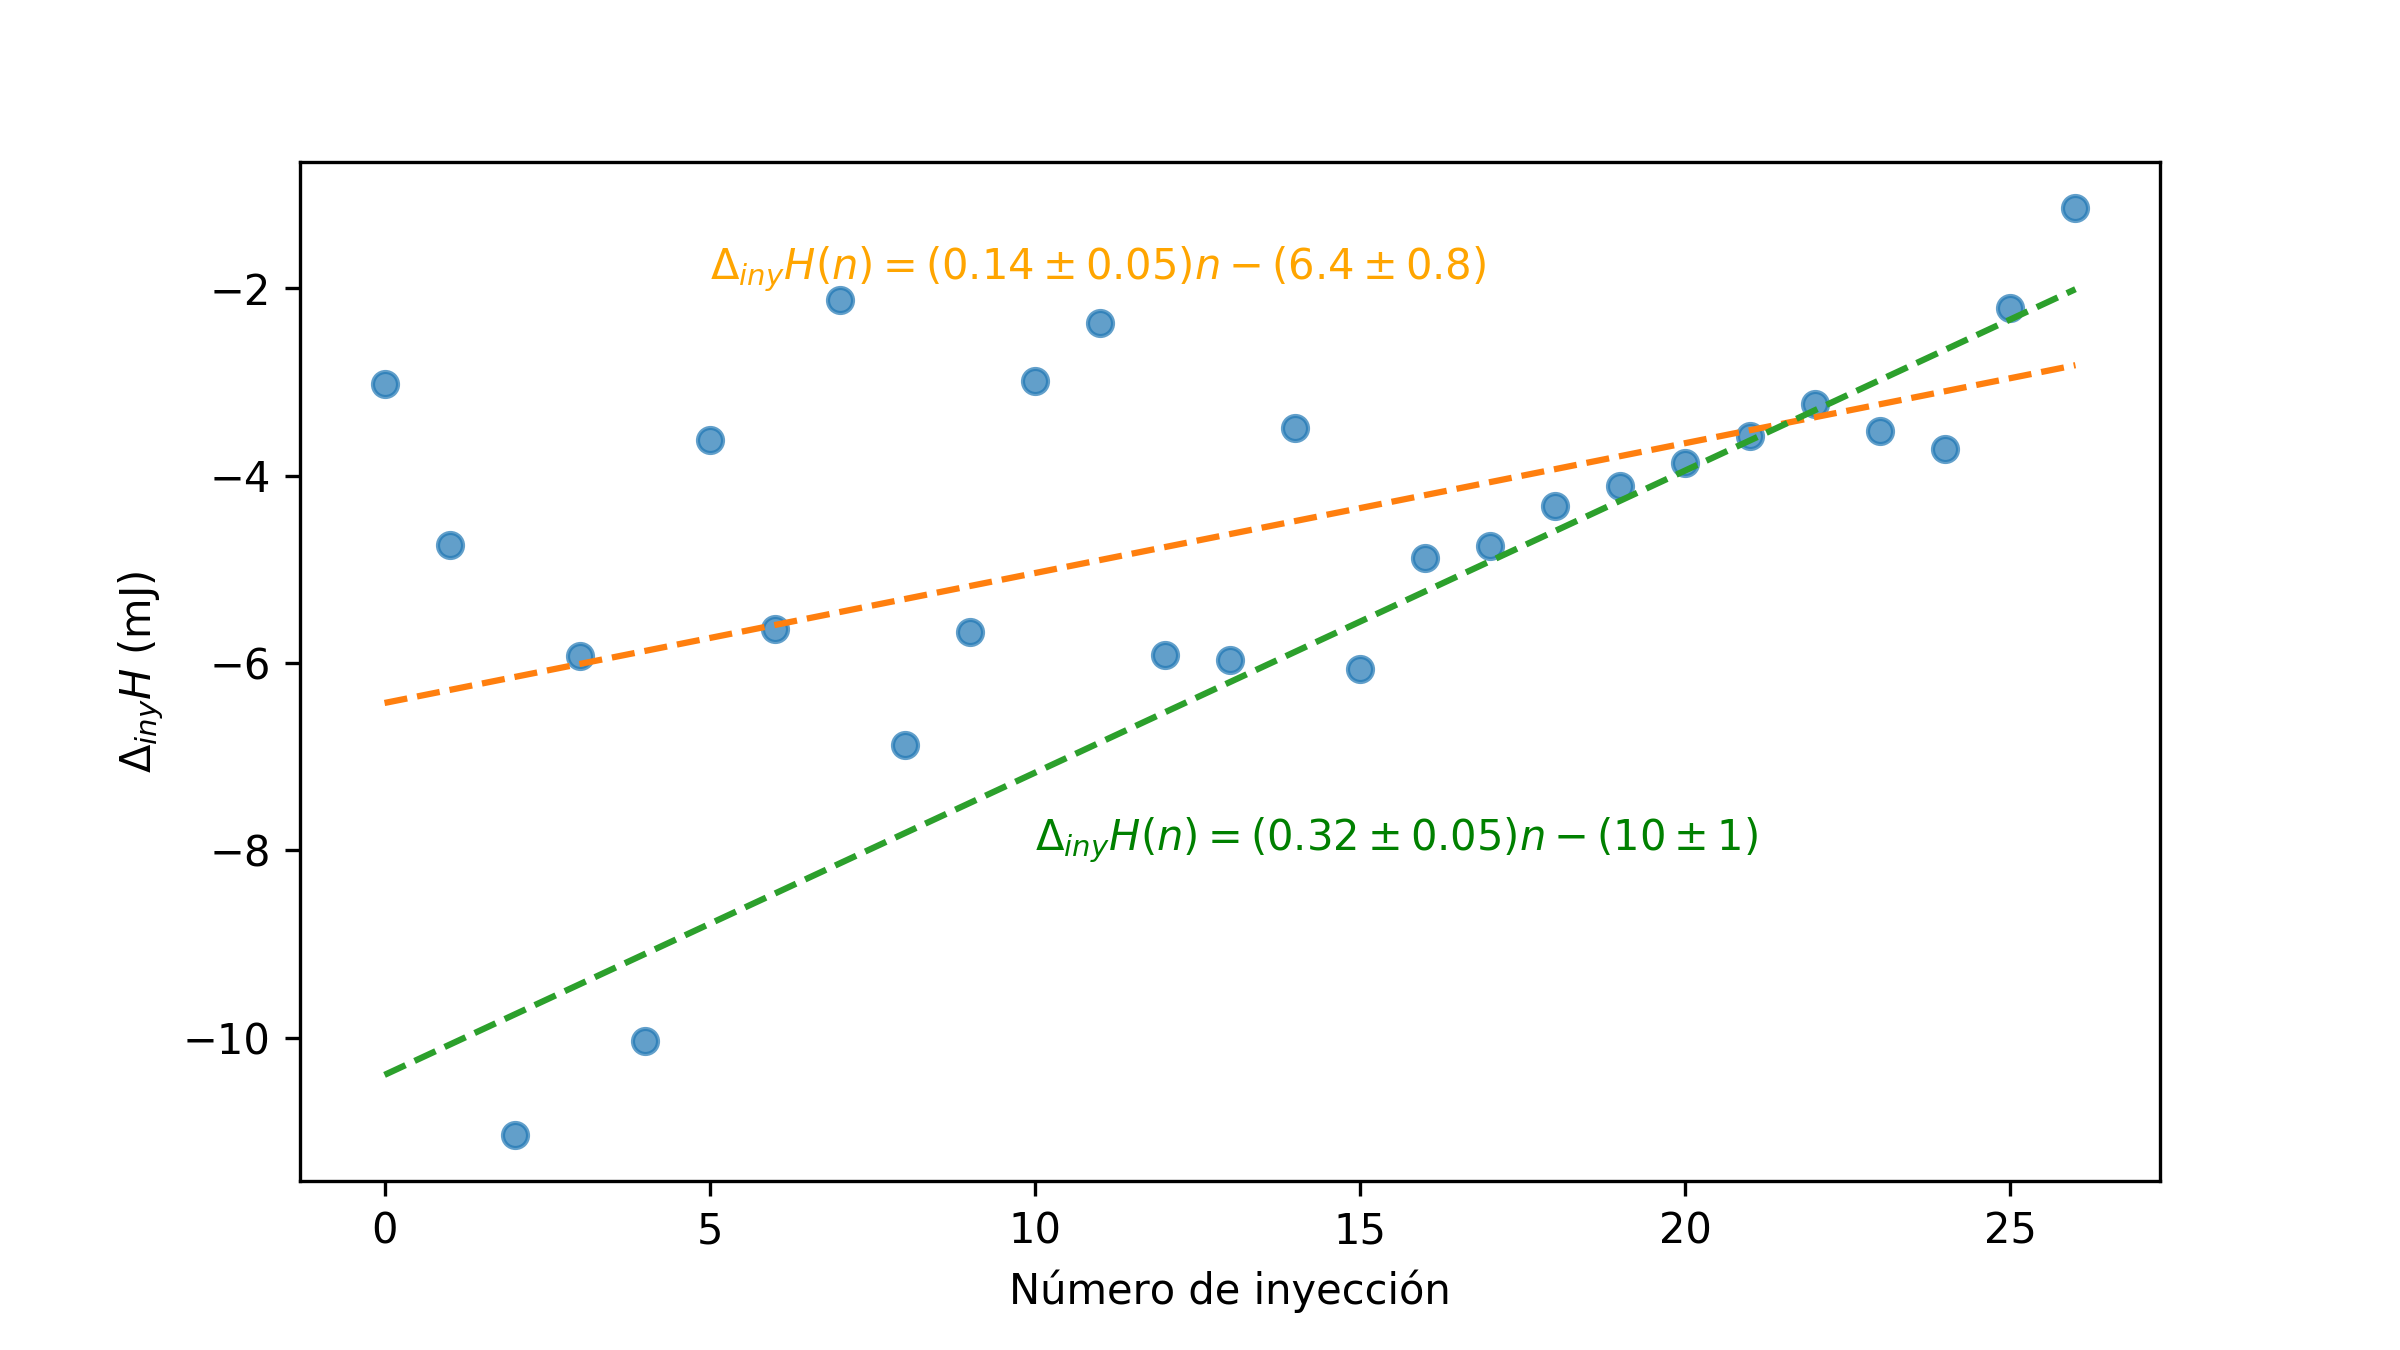
\includegraphics[width=0.53\linewidth]{../Data/ChemicalCalibrations/multipleInt}
		\end{tabular}
		\caption{Resultados con inyecciones m\'ultiples de 1-propanol al 2.96 \% (p/p).}
	\end{figure}

	Para la reacci\'on \'acido base se prepar\'o una soluci\'on 0.247 mM de HCl, diluyendo 1.0 mL de una soluci\'on de HCl concentrada en 25 mL de agua, de esta soluci\'on se tomaron 0.0297 g los cuales se disolvieron en 99,5553 g de agua. Para el \ce{KHCO3} se agregaron 0.10143 g de \ce{KHCO3} a 9.93551 g de agua, y se diluyeron 0.1709 g de esta soluci\'on, en 99,5657 g de agua.

	\begin{figure}[h]
		\centering
		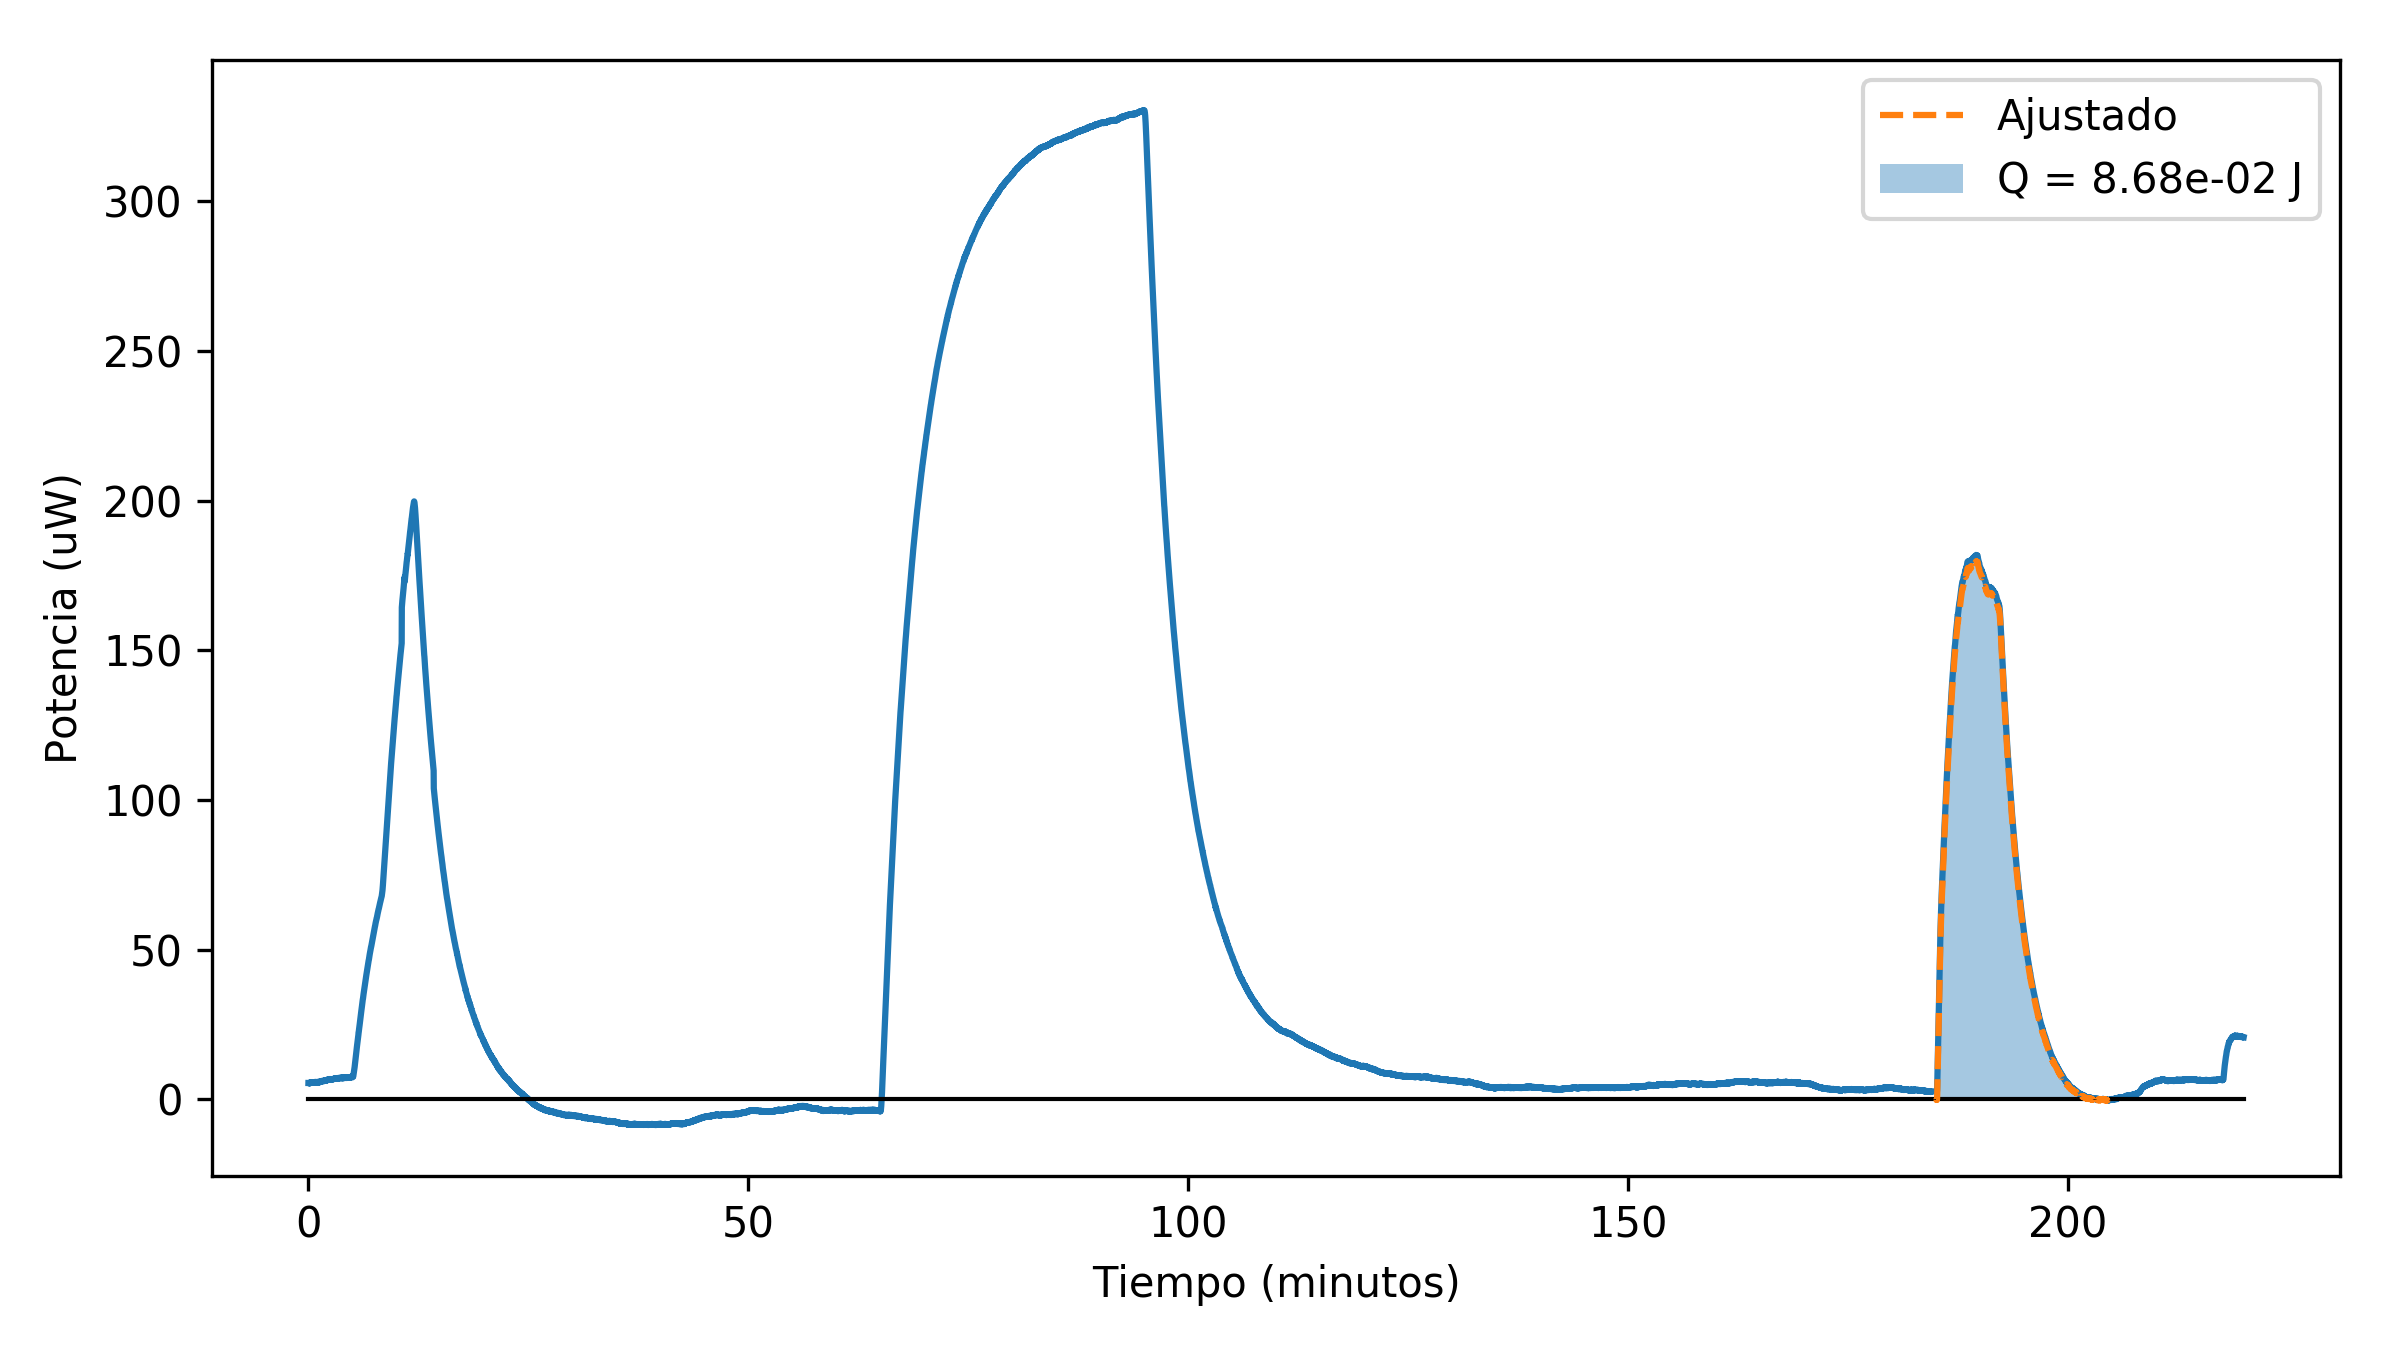
\includegraphics[width=\figwidth]{../Data/ChemicalCalibrations/HCl}
		\caption{Resultados para la neutralización del {KHCO3}, $\Delta H$ = -254 kJ/mol.}
	\end{figure}

	\begin{equation}
		\ce{KHCO3(ac) + HCl(ac) <=>[K_a] H2O(l) + KCl(ac) + CO2(g)}
	\end{equation}

	Usando la entalp\'ia reportada para la reacci\'on anterior se calcul\'o el factor calorim\'etrico en 28.
	
\section{Conclusiones}
	Se realiz\'o la instalaci\'on del calorímetro adaptando el equipo a la red eléctrica colombiana. Además, se logró la comunicaci\'on del calor\'imetro con el computador eliminando la necesidad de puertos RS232, el funcionamiento del agitador fue optimizado al sustituir la conexión original a un puerto USB, y se caracteriz\'o el efecto del mismo sobre las lecturas calorim\'etricas. Los parámetros usados para estabilizar el calorímetro a 25 \grad{} fueron reportados, y se encontró el factor calorimétrico en 28, con el cual la entalpía de mezcla del 1-propanol fue de -7.89 y -7.18 kJ/mol, respectivamente.

\printbibliography[heading=bibintoc, title={Referencias}]
\section*{Agradecimientos}
	Al profesor Edgar Vargas por su confianza y apoyo, y a Nicol\'as Moreno y Valeria Eslava por su buena disposici\'on.
\end{multicols}
\end{document}